\documentclass{scrartcl}
\usepackage[utf8]{inputenc}
\usepackage[T1]{fontenc}
\usepackage[ngerman]{babel}
\usepackage{amssymb}
\usepackage{amsmath}
\usepackage{graphicx}
\usepackage{framed}
\usepackage{xcolor}
\usepackage[nottoc]{tocbibind}
\usepackage{caption}

\colorlet{shadecolor}{gray!25}
\setlength{\parindent}{0pt}

\newcommand{\abs}[1]{\left\lvert#1\right\rvert}

\begin{document}
% ----------------------------------------------------------------------
\title{Approximation von Ableitungen\\mittels finiter Differenzen}
\author{Marisa Breßler und Anne Jeschke}
\date{08.11.2019}
\maketitle
% ----------------------------------------------------------------------------
% Inhaltsverzeichnis:
\tableofcontents
% ----------------------------------------------------------------------------
% Gliederung und Text:
\pagebreak \section{Einleitung}
\label{sec:einleitung}
Im Gegensatz zur Analysis bietet die Numerik in der Praxis anwendbare Lösungen von Problemen und ermöglicht Näherungen an Real- bzw. Idealbilder. Die Güte dieser Näherung ist abschätzbar, bleibt also also unterhalb einer beweisbaren Toleranzgrenze. \\
Wieso müssen wir Ableitungen approximieren? Ableitungen von Funktionen spielen in der Praxis eine große Rolle. So dienen zum Beispiel die erste und zweite Ableitung in der Physik der Untersuchung von Bewegungsabläufen. Hier werden die Geschwindigkeit und Beschleunigung als erste und zweite Ableitung des Weges nach der Zeit definiert. Änderungsprozesse müssen in ganz unterschiedlichen Kontexten erfasst und/oder vorausgesagt werden. Dabei ist es in einer Vielzahl von Praxisbeispielen notwendig, Ableitungen zu approximieren. Denn unter Umständen ist eine Funktion zwar durch Formeln bekannt, doch das exakte Differenzieren gestaltet sich als aufwändig oder das Ermitteln von Funktionswerten als schwierig, weil die Ableitungsfunktion von sehr komplexer Natur ist. Das numerische Differenzieren hat eines seiner Hauptanwendungsgebiete in der Verarbeitung von Messdaten. Hier ist die Funktion im Allgemeinen nicht explizit bekannt, das heißt sie liegt nicht in analytischer Form vor, sondern nur in Form von diskreten Werten. Aufgrund der gegebenen lückenhaften Informationen ist die Ableitung mit analytischen Methoden der Differentialrechnung nicht exakt bestimmbar. An dieser Stelle werden numerische Verfahren verwendet, um die Ableitungen, beziehungsweise die Werte der Ableitungen an bestimmten Stellen, mit einer gewissen Genauigkeit näherungsweise zu ermitteln. \\
\linebreak
\textit{Numerik beantwortet die Frage: Was bleibt vom Ableitungsbegriff übrig, wenn alle Rechnungen in endlich vielen Schritten und mit endlich vielen Zahlen in endlich vielen Ziffern abgehandelt werden müssen?}\cite{schneebeli}\\
\linebreak
Numerisches Differenzieren ist zum Beispiel mit den sogenannten finiten Differenzen möglich. Diese stellen eine überschaubares Verfahren zum Approximieren von Ableitungen zur Verfügung. Auf welche Weise und wie gut, das heißt mit welcher Genauigkeit, das funktioniert, soll im Folgenden erläutert werden. \\

\pagebreak \section{Theorie}
\label{sec:theorie}
Die Formeln der finiten Differenzen, auch Differenzenformeln genannt, lassen sich auf verschiedene Weisen herleiten. Im Folgenden wollen wir zwei Ansätze vorstellen: Zum einen ist das ein geometrischer Ansatz, der die Definition der Ableitung über den Differentialquotienten nutzt, d.h. den Anstieg der Tangente an der zu untersuchenden Funktion an der zu betrachtenden Stelle. Zum anderen ist es ein analytischer Ansatz, der sich die Eigenschaften der Taylorentwicklung zunutze macht.

\subsection{Vom Differential- zum Differenzenquotienten und umgekehrt}
\label{ssec:herleitung1}
Der Ausgangspunkt unserer geometrischen Herleitung der Differenzenformeln bildet die Definition der Ableitung:
\begin{shaded}
Eine Funktion $f:D \rightarrow \mathbb{R}$ (mit $D\subset \mathbb{R}$) heißt differenzierbar an der Stelle $x_0 \in D$, falls folgender Grenzwert existiert (mit $(x_0+h) \in D$): \[f'(x_0) = \lim _{x\to x_0} {\frac {f(x)-f(x_0)}{x-x_0}} = \lim _{h\to 0} {\frac {f(x_0+h)-f(x_0)}{h}}\] Dieser Grenzwert heißt \textit{Differentialquotient} / \textit{Ableitung} von $f$ nach $x$ an der Stelle $x_0$.
\end{shaded}
Der Differentialquotient geht zurück auf die Sekantensteigung. Ist die Ableitung einer Funktion $f$ an einer Stelle $x_0$ gesucht, wird wie eingangs erwähnt nach der Steigung der Tangente am Graphen von $f$ im Punkt $(x_0 \mid f(x_0))$ gefragt. Die Tangentensteigung kann näherungsweise mit der Sekantensteigung durch die zwei Punkte $(x_0 \mid f(x_0))$ und $(x_0 + h \mid f(x_0 + h))$ bestimmt werden (wobei $0<h \in \mathbb{R}$). Die Formel der Sekantensteigung durch eben diese Punkte ist der folgende Differenzenquotient: \[\frac {f(x_0 + h)-f(h)}{(x_0 + h) - x_0} = \frac {f(x_0 + h)-f(h)}{h}\]
Verkleinert man die sogenannte \textit{Schrittweite} $h$ immer mehr, kommt die Sekantensteigung der Tangentensteigung immer näher. Lässt man $h$ also gegen $0$ laufen, erhält man die Formel für den Differentialquotienten, sprich für die Ableitung von $f$ an der Stelle $x_0$. Allerdings kann der Computer den Grenzübergang von $h$ gegen $0$ nicht leisten. Deswegen wählt man den Differenzenquotienten als Näherung der Ableitung. Werden Rundungsfehler vernachlässigt, die ein Computer aufgrund seiner begrenzten Genauigkeit in der Zahldarstellung verursacht (siehe hierzu Abschnitt 2.3), geht der numerische Wert des Differenzenquotienten gegen den exakten Wert der Ableitung. In der Praxis gilt die Faustregel: Je kleiner die Schrittweite $h$ gewählt wird, desto genauer ist die numerische Näherung. \\
Der Differenzenquotient misst die mittlere spezifische Änderung von $f$ zwischen $x_0$ und einer zweiten nahe liegenden Stelle. Man unterscheidet zwischen dem \textit{rechtsseitigem Differenzenquotienten}, bei dem die Steigung der Sekante durch $x$ und $x_0 + h$ berechnet wird, und dem \textit{linksseitigen Differenzenquotienten}, bei dem wiederum die Steigung der Sekante durch $x_0 - h$ und $x$ berechnet wird. Allerdings ist die Nutzung des links- oder des rechtsseitigen Differenzenquotienten, einer \textit{finiten Differenz erster Ordnung} suboptimal, vor allem für einseitig gekrümmte Funktionsgraphen, bei denen oft eine sehr hohe Abweichung zwischen Sekanten- und Tangentensteigung zu beobachten ist. Deshalb kann es unter Umständen sinnvoll sein, diesen Fehler durch Mittelung zu verkleinern und das arithmetische Mittel der beiden einseitigen (asymmetrischen) Differenzenquotienten zu betrachten, das heißt die Sekantensteigung zwischen $x_0 - h$ und $x_0 + h$. Dies bezeichnet man als \textit{zentralen} oder auch \textit{symmetrischen Differenzenquotienten erster Ordnung}. Durch erneutes Anwenden der symmetrischen Differenzenformel für die erste Ableitung lässt sich eine symmetrische Differenzenformel zur Approximation der zweiten Ableitung gewinnen: der \textit{symmetrische Differenzenquotient zweiter Ordnung} bzw. die \textit{zweite finite Differenz}. Für höhere Ableitungen geht man analog vor.\cite{westermann}
\begin{shaded}
\begin{center}
 rechtsseitiger Differenzenquotient / finite Differenz erster Ordnung:
 \end{center} \[ \frac {f(x_0 + h) - f(x_0)}{h} \]
\begin{center}
 linkssseitiger Differenzenquotient / finite Differenz erster Ordnung:
 \end{center} \[ \frac {f(x_0) - f(x_0 - h)}{h} \]
\begin{center}
 zentraler Differenzenquotient erster Ordnung:
 \end{center} \[ \frac {f(x_0 + h) - f(x_0-h)}{2h} \]
\begin{center}
 zentraler Differenzenquotient zweiter Ordnung / zweite finite Differenz:
 \end{center} \[ \frac{f(x_0+h) - 2f(x_0)+f(x_0-h)}{h^2} \]
\end{shaded}

\subsection{Approximieren von Ableitungen via Taylorentwicklung}
\label{ssec:herleitung2}
Auch mit Hilfe der Taylorentwicklung einer Funktion lassen sich Formeln zur Approximation der Ableitungen einer Funktion herleiten. Betrachtet man auf einem Intervall $[a,b] \in \mathbb{R}$ eine reelle Funktion $f \in C^\infty([a,b])$, so kann man die Ableitung an einer Stelle $x \in (a,b)$ annähernd bestimmen, indem man zusätzlich eine in der Nähe liegende Stelle $(x+h) \in [a,b]$ mit $0<h \in \mathbb{R}$ betrachtet und den Funktionswert von $f$ an dieser Stelle als Taylorreihe von $f$ mit Entwicklungsstelle $x+h$ darstellt:
\[f(x+h) = \sum_{n=0}^{\infty}\frac{f^{(n)}(x)}{n!}h^n = f(x)+f'(x)h+\frac{f''(x)}{2}h^2+...\]
Wenn man diese Formel entsprechend äquivalent umformt (Subtraktion von $f(x)$ und Dividieren von $h$), erhält man die Formel für die \textbf{\textit{erste finite Differenz}} von $f$ an der Stelle $x$:
\begin{shaded}
\[(D_h^{(1)}f)(x) = \frac{f(x+h)-f(x)}{h} = f'(x)+\frac{f''(x)}{2}h+...=f'(x)+\mathcal{O}(h)\;\]
\end{shaded}
Die erste finite Differenz von $f$ an der Stelle $x$ entspricht also bis auf eine lineare Restgliedabschätzung der ersten Ableitung von $f$ an der Stelle $x$. \\
Auch die zweite Ableitung von $f$ an der Stelle $x$ können wir auf ähnliche Weise mittels Funktionswerten von $f$ approximieren. Dazu benötigen wir zusätzlich die Taylorreihe von $f$ mit Entwicklungsstelle $(x-h) \in [a,b]$, die ebenfalls in der Nähe von $x$ liegt:
\[f(x-h) = \sum_{n=0}^{\infty}\frac{f^{(n)}(x)}{n!}(-h)^n = f(x)-f'(x)h+\frac{f''(x)}{2}h^2+...\]
Durch Aufsummieren der beiden Formeln für die Taylorentwicklung um $x+h$ und $x-h$ und Äquivalenzumformungen (Subtraktion von $2f(x)$ und Dividieren von $h^{2}$) erhält man die Formel für die \textbf{\textit{zweite finite Differenz}} von $f$ an der Stelle $x$:
\begin{shaded}
\[(D_h^{(2)}f)(x) = \frac{f(x+h)-2f(x)+f(x-h)}{h^2} = f''(x)+\frac{f^{(4)}(x)h^2}{3\cdot4}+...=f''(x)+\mathcal{O}(h^2)\;\]
\end{shaded}
Diese entspricht wiederum bis auf eine quadratische Restgliedabschätzung der zweiten Ableitung von $f$ an der Stelle $x$.\cite{ppi}

\subsection{Fehler und Schrittweite}
\label{ssec:schrittweite}
Die Fehler numerischer Berechnungen gegenüber exakter analytischer setzen sich ganz allgemein zusammen aus \textit{Verfahrensfehlern} und \textit{Rundungsfehlern}.\cite{westermann} Der Verfahrensfehler gibt bezogen auf numerisches Differenzieren in der hier besprochenen Form den Unterschied zwischen dem exakten Wert der Ableitung an der Stelle $x$ und dem exakten Wert des Differenzenquotienten an der Stelle $x$ an. Rundungsfehler sind hingegen darauf zurückzuführen, dass der Computer aufgrund eines begrenzten Speichers Zahlen nur mit endlicher Genauigkeit darstellen und verarbeiten kann. Er verfügt lediglich über einen endlichen Vorrat an sogenannten Maschinenzahlen. Gibt der Benutzer eine Zahl in den Computer ein, die keine Maschinenzahl ist, wird sie zur nächstgelegenen Maschinenzahl gerundet. So kommt es insbesondere in dem Bereich der reellen Zahlen bereits bei der Übergabe von Zahlen an den Computer zu Rundungsfehlern. Aber auch nach jeder Operation rundet die Maschine und produziert damit weitere Rundungsfehler. Die Verstärkung der Rundungsfehler wird als \textit{Fehlerfortpflanzung} bezeichnet. Wie problematisch diese Fehler sind, ist von den Zahlen, der Art und der Reihenfolge der ausgeführten Operationen abhängig. In der Computerarithmetik sind Addition und Multiplikation zwar kommutativ, jedoch gelten Assoziativ- und Distributivgesetze im Allgemeinen nicht. Demnach können analytisch äquivalente Ausdrücke auf dem Computer zu erheblich unterschiedlichen Ergebnissen führen.\cite{nla} \\
Ein heikler Punkt bei der Approximation der Ableitungen mit Differenzenquotienten ist die Wahl der Schrittweite $h$. Ein zu großes $h$ führt zu Verfahrensfehlern, ein zu kleines $h$ birgt die Gefahr der \textit{Auslöschung}. Die Subtraktion fast gleich großer Zahlen (die wir bei unseren Differenzenformeln für die erste und zweite Ableitung im Zählerterm finden) kann dazu führen, dass die Differenz zwischen den beiden Zahlen für den Computer nicht mehr erfassbar ist und signifikante Stellen \textit{ausgelöscht} werden.\cite{am}
So wird der Approximationsfehler beim Vermindern der Schrittweite zunächst kleiner, da die Funktionalität des Verfahrens und damit die Genauigkeit der Näherung steigt.
Allerdings macht sich im Laufe der Zeit die eben benannte Grenze bemerkbar. Bei sehr kleinen Schrittweiten muss mit Auslöschung gerechnet werden und damit wieder mit einer sinkenden Genauigkeit.\cite{schneebeli}
Ist das Ziel, möglichst genau zu approximieren, sollte man dieses "`optimale"' $h$, ab dem die Genauigkeit der Näherung mit dem Verkleinern der Schrittweite nicht weiter zunimmt, ausfindig machen. Unter Umständen genügen aber bereits gröbere Näherungen und andere Faktoren spielen eine wichtigere Rolle. \\

\pagebreak \section{Experimente und Beobachtungen}
\label{sec:experimente}

Wir betrachten zunächst die Funktion $g_1:[\pi, 3\pi] \rightarrow \mathbb{R}$ mit $g_1(x) = sin(x)/x$. Mit Hilfe eines in Python verfassten Programmes, das als "`serie1\_experimente.py"' zusammen mit diesem Bericht eingereicht wird, lassen wir folgende Graphen zeichnen:
Den von $g_1$, den der exakten ersten und zweiten Ableitung $g_1': [\pi, 3\pi] \rightarrow \mathbb{R}$ mit $g_1'(x) = \frac{x \cdot cos(x) - sin(x)}{x^{2}}$ und $g_1'': [\pi, 3\pi] \rightarrow \mathbb{R}$ mit $g_1''(x) = \frac{-2x \cdot cos(x) + (2-x^{2}) sin(x)}{x^{3}}$, die wir nach den analytischen Methoden der Differentialrechnung ermittelt haben, sowie den der ersten finiten Differenz $D_h^{(1)}g$ und den der zweiten $D_h^{(2)}g$.
Für die Auswertung der genannten Funktionen durch den Computer unterteilen wir den Definitionsbereich $[\pi, 3\pi]$ in $p = 1000$ äquidistante Intervalle.
Nur an den Intervallgrenzen $x_i$ (mit $i \in \lbrace 0, 1, 2, ..., p \rbrace$) soll ausgewertet werden. \\
\\
Nun wollen wir die exakte und die approximierte erste und zweite Ableitung von $g_1$ für die Schrittweiten $h = \pi/3$, $h = \pi/4$, $h = \pi/5$ und $h = \pi/10$ graphisch vergleichen. \\
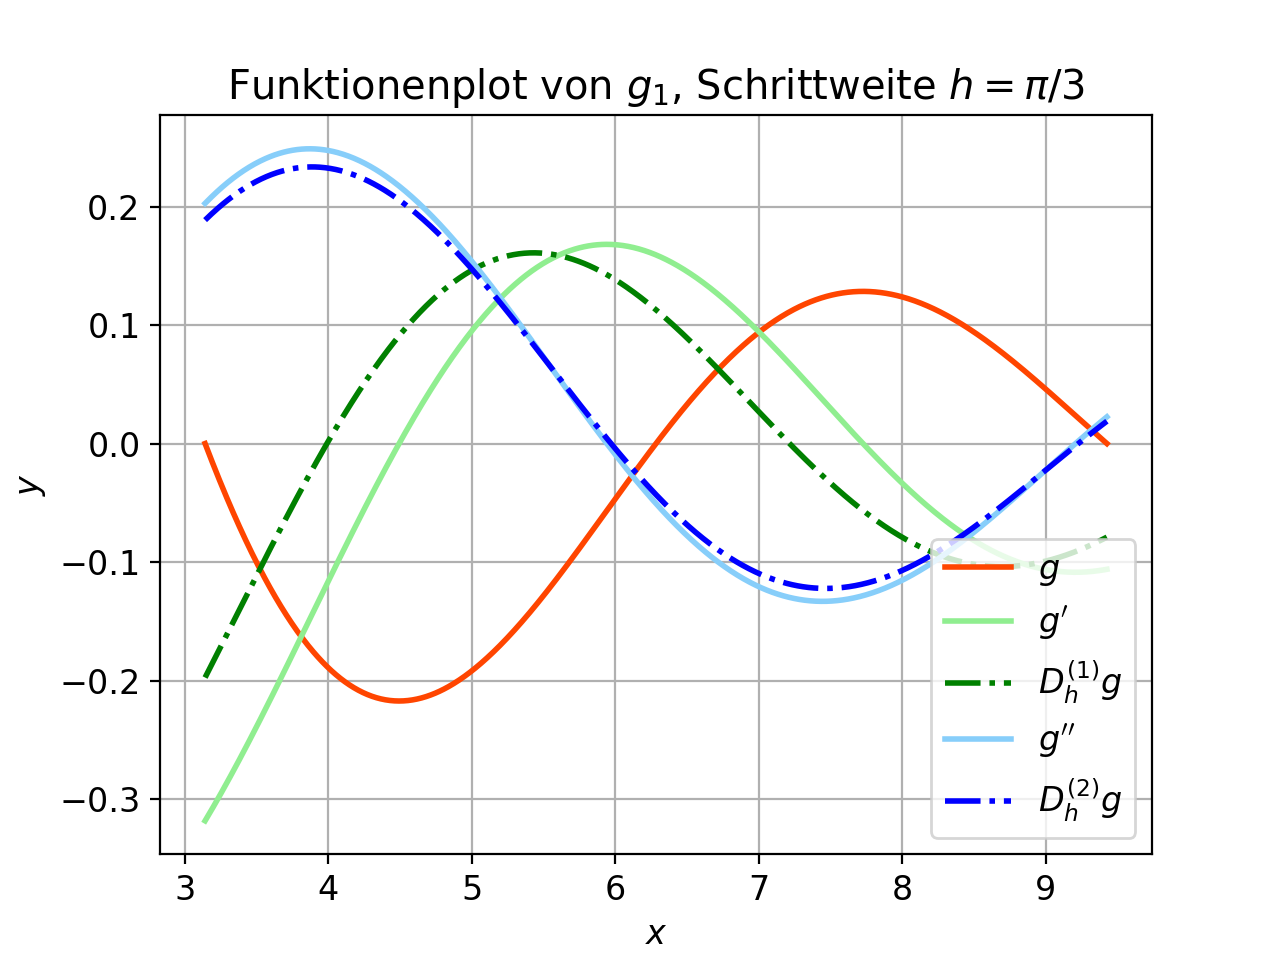
\includegraphics[width=0.5\textwidth]{Grafiken/Funktionenplot_Pi_Drittel} 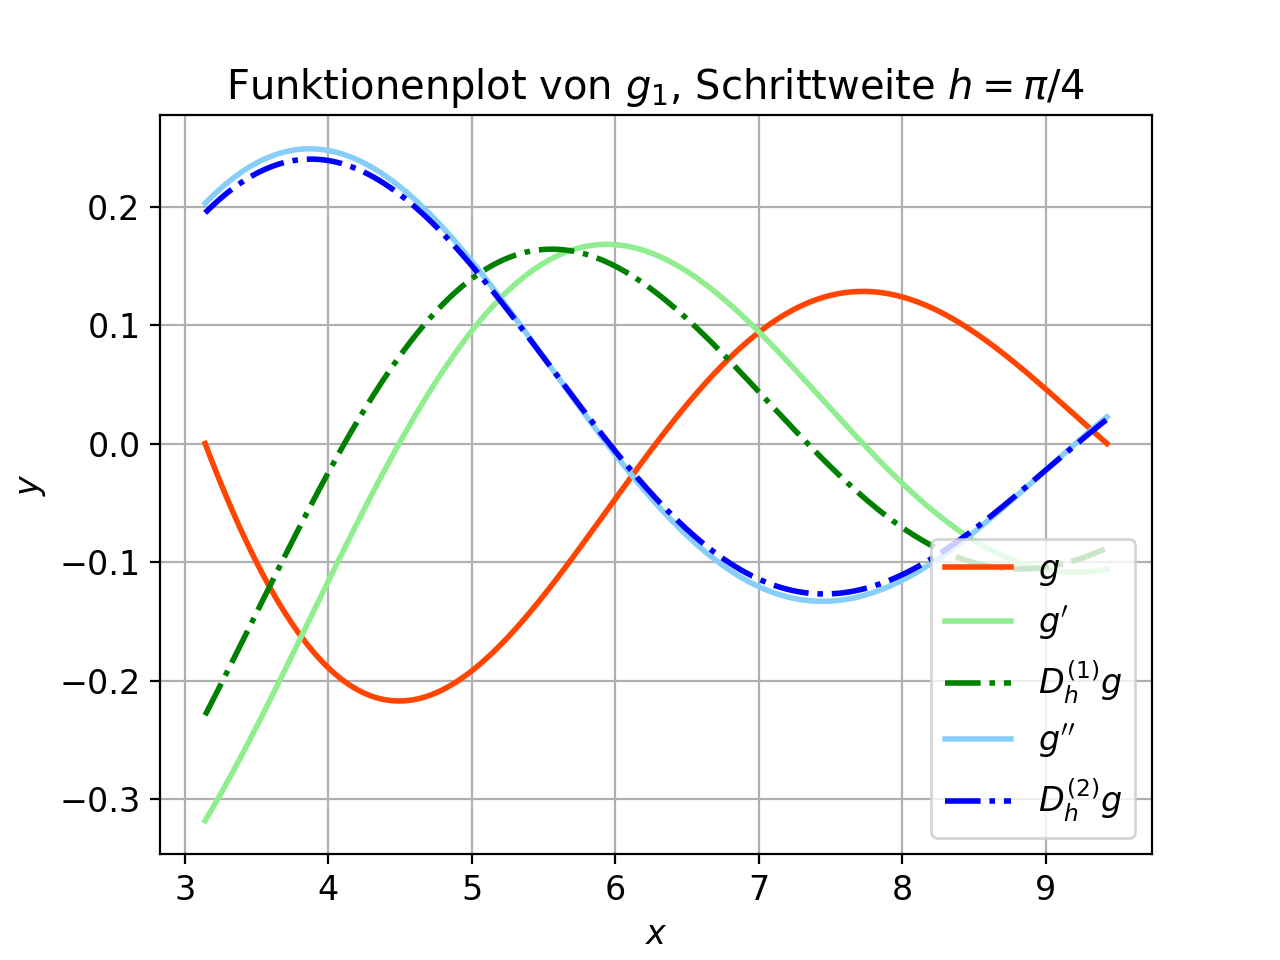
\includegraphics[width=0.5\textwidth]{Grafiken/Funktionenplot_Pi_Viertel}\\
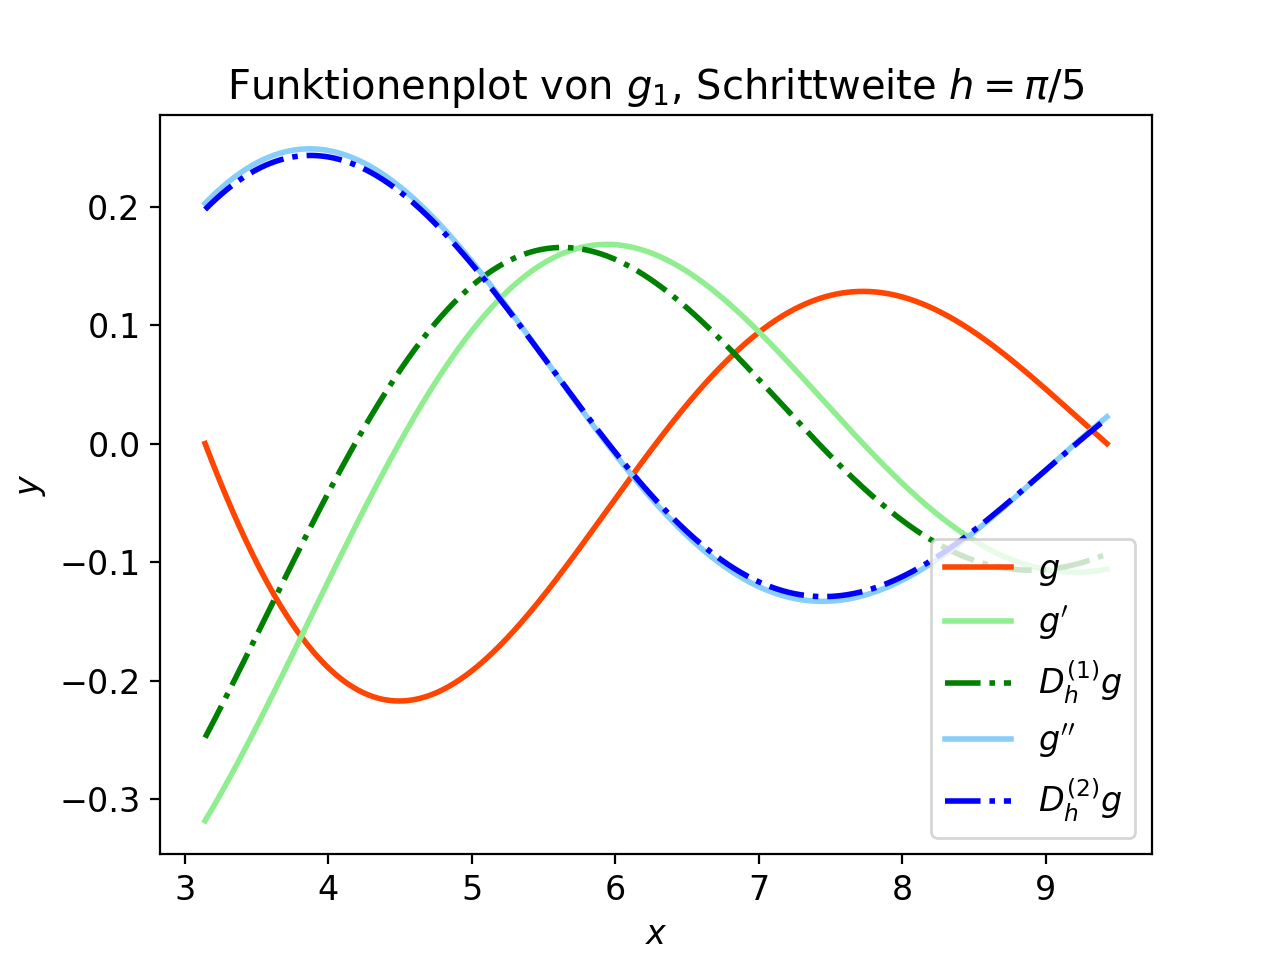
\includegraphics[width=0.5\textwidth]{Grafiken/Funktionenplot_Pi_Funftel} 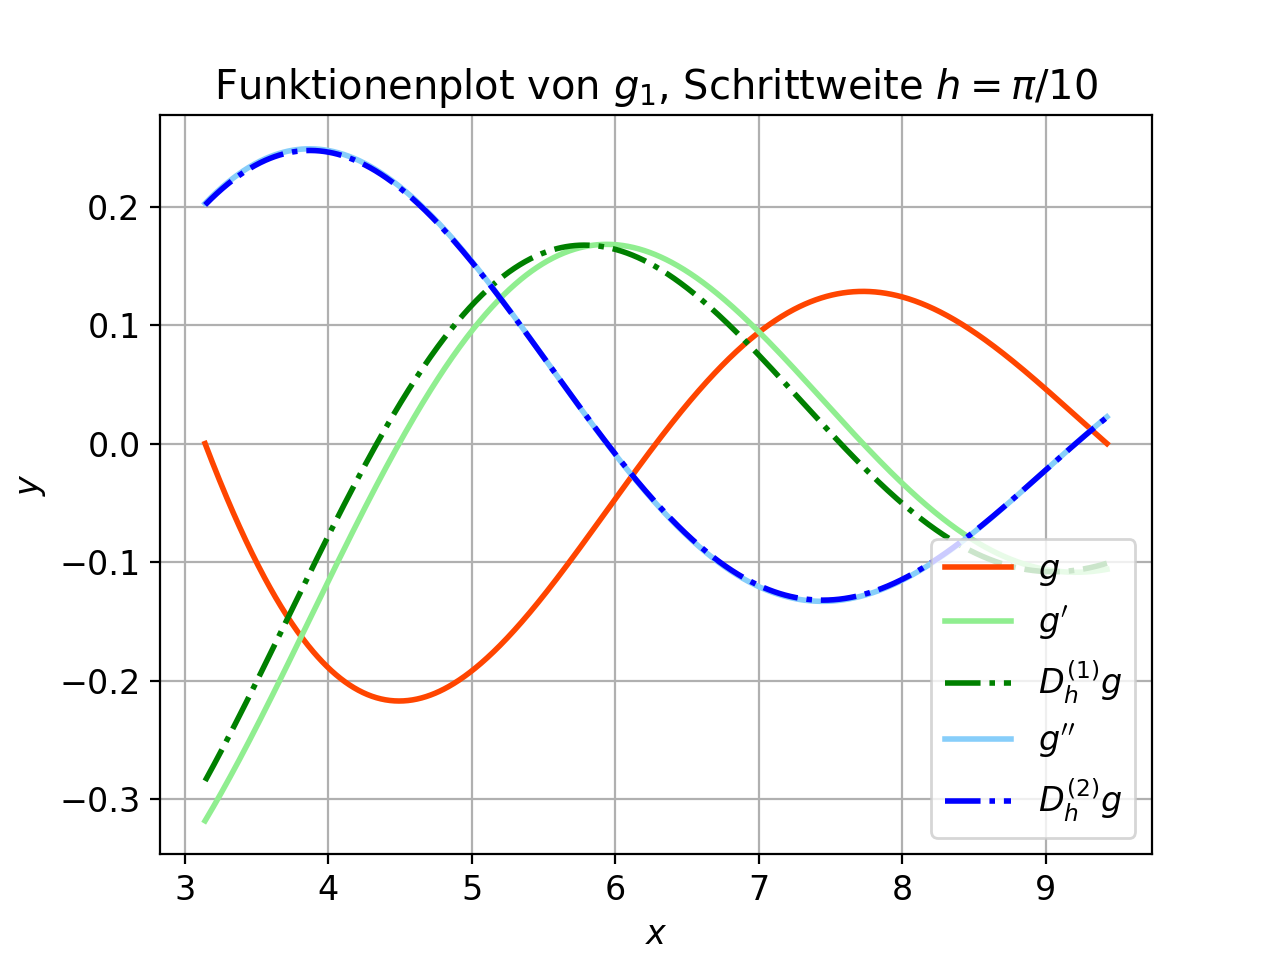
\includegraphics[width=0.5\textwidth]{Grafiken/Funktionenplot_Pi_Zehntel}\\
\vspace{-0.5cm}
\captionof{figure}{Funktionsplots von $g_1$ mit unterschiedlichen Schrittweiten}
\vspace{0.5cm}
Allgemein ist folgender Zusammenhang erkennbar: Je kleiner die Schrittweite, desto besser die Approximation.
Darüber hinaus fällt auf, dass für alle $h$ die Näherung der jeweiligen Ableitung mittels zweiter finiter Differenz besser als die mittels erster finiter Differenz.
Bereits mit der gröbsten Schrittweite $h = \pi/3$ ist die Approximation der zweiten Ableitung gut.
Eine vergleichbar gute Approximation der ersten Ableitung erhalten wir erst mit der feinsten Schrittweite $h = \pi/10$.
Bei dieser Schrittweite liegt der Graph der approximierten zweiten Ableitung bereits so gut wie auf dem Graphen der exakten. \\
 \\
Um das Konvergenzverhalten der Finite-Differenzen-Verfahren exemplarisch für die erste und zweite Ableitung graphisch zu untersuchen, lassen wir bei gleich bleibenden Parametern ($g_1$, $[\pi, 3\pi]$, $p = 1000$) die maximalen absoluten Fehler in Abhängigkeit von der Schrittweite $h$ in einem Fehlerplot ausgeben, wobei die Referenzwerte die exakten Ableitungen zur Verfügung stellen. Dabei bezeichne $e_g^{(1)}$ den Fehler bei der ersten finiten Differenz und $e_g^{(2)}$ den Fehler bei der zweitem finiten Differenz. Wir betrachten die Approximationsfehler in der Maximumnorm mit der Formel (wobei die $x_i$'s die Intervallgrenzen unserer äquidistanten Unterteilen sind):
\[e_g^{(k)}(h):=\max_{i=0,..,p}\abs{g^{(k)}(x_i)-(D_h^{(k)}g)(x_i)} , k \in \lbrace1, 2\rbrace\]
Folgende Werte für $h$ sollen ausgewertet werden: $10^{-10}$, $5 \cdot 10^{-10}$, $10^{-9}$, $5 \cdot 10^{-9}$, ... , $10^{-1}$, \linebreak  $5 \cdot 10^{-1}$, $1$, $5$, $10$.
Um in der Grafik erkennen zu können, mit welcher Geschwindigkeit sich die maximalen Approximationsfehler ändern, lassen wir zudem die Graphen von $h \mapsto h$, $h \mapsto h^{2}$ und $h \mapsto h^{3}$ zeichnen und wählen die Darstellung in einem doppeltlogarithmischen Plot.
\begin{center}
	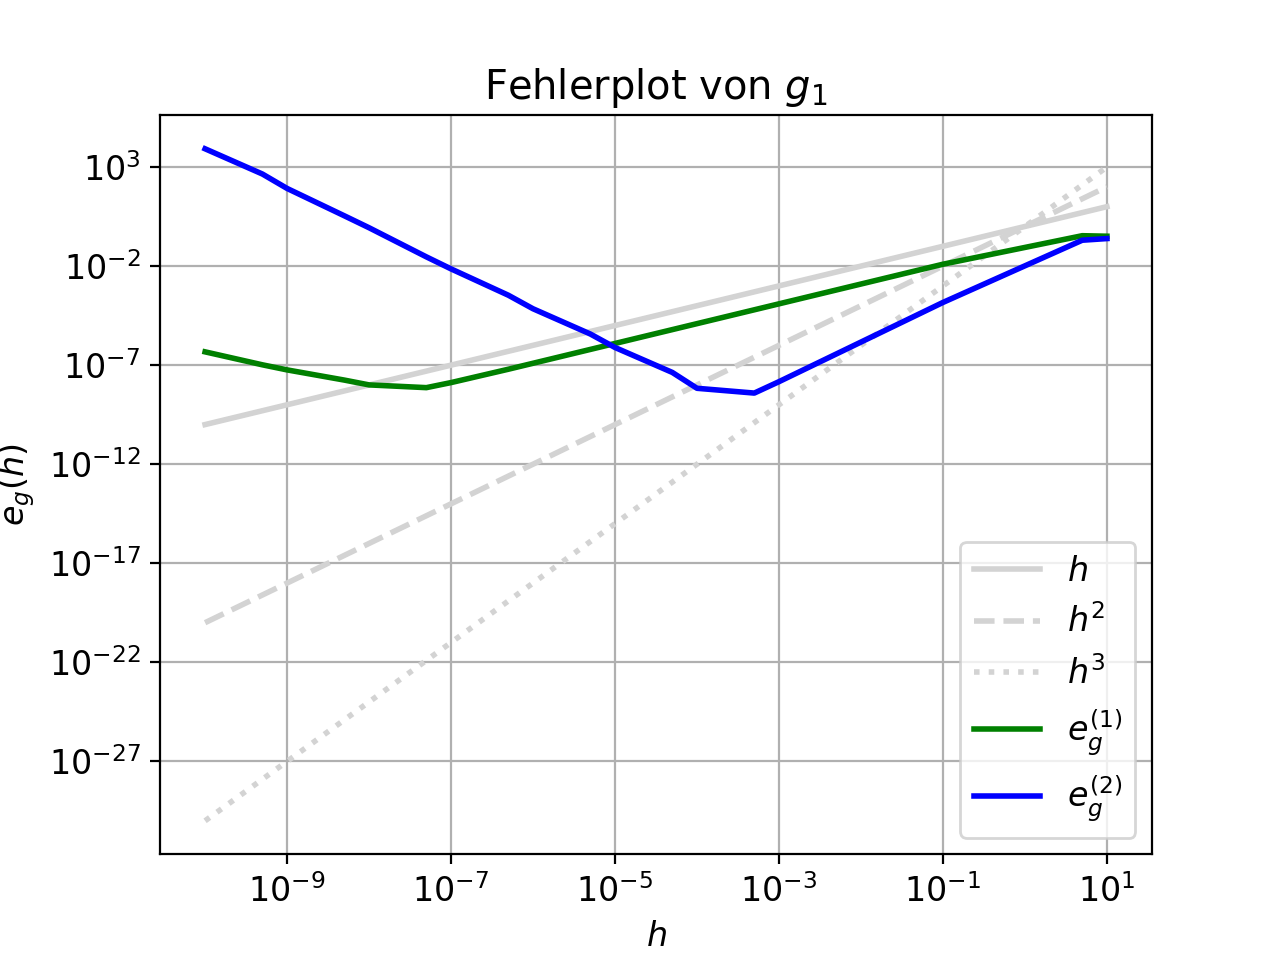
\includegraphics[width=0.65\textwidth]{Grafiken/Fehlerplot_Aufgabe2}
  \vspace{-0.2cm}
  \captionof{figure}{Fehlerplot von $g_1$}
  \vspace{0.5cm}
\end{center}
Es lässt sich beobachten, dass sowohl der maximale Fehler der ersten finiten Differenz als auch der der zweiten finiten Differenz in einer Größenordnung von etwa $0.5$ starten (für eine sehr grobe Schrittweite $h \approx 5$). Mit zunehmend kleinem $h$ nimmt auch der Approximationsfehler ab. Dabei wird der Fehler bezüglich der ersten Ableitung linear kleiner und bezüglich der zweiten Ableitung quadratisch. Jedoch nimmt er ab einer gewissen Schrittweite $h$ wieder zu. Für die erste finite Differenz ist das ab $h = 5\cdot10^{-8}$, für die zweite finite Differenz ist das bereits ab $h = 5 \cdot 10^{-4}$ der Fall (für beide: $e_g(h) \approx  5 \cdot 10^{-9}$). Nun nimmt der Fehler mit ähnlicher Geschwindigkeit zu, wie er vormals abgenommen hat. Mit der feinsten Schrittweite von $h = 10^{-10}$ liegt der maximale Fehler der erstem finiten Differenz immer noch gut bei $5 \cdot 10^{-7}$, während der maximale Fehler der zweiten finiten Differenz mit einer Größenordnung von $10^{4}$ sehr stark angewachsen ist. \\
 \\
In weiterführenden Experimenten wollen wir die Funktion $g_j:[\pi, 3\pi] \rightarrow \mathbb{R}$ mit $g_j(x) = sin(j x)/x$. Wieder haben wir die erste und die zweite Ableitung mit analytischen Methoden der Differentialrechnung ermittelt:

\begin{center}
$g_j'(x) = \frac{jx \cdot cos(jx) - sin(jx)}{x^{2}}$ und $g_j''(x) = \frac{-2jx \cdot cos(jx) + (2-j^{2}x^{2}) sin(jx)}{x^{3}}$
\end{center}

Zunächst wählen wir $j>1$ und anschließend $j<1$ ($j \in \mathbb{R^{+}}$). Im Vergleich zu $j = 1$ bewirken größere $j$'s eine Stauchung des ursprünglichen Graphen in $x$-Richtung. Kleinere $j$'s bewirken das Gegenteil, eine Streckung des ursprünglichen Graphen in $x$-Richtung. Während immer größere $j$'s die Frequenz von $g_j$ erhöhen, kommt es bei immer kleineren $j$'s zum Vermindern der Frequenz. Das heißt, dass sich die Funktionswerte von $g_j$ auf demselben Intervall bei größeren $j$'s schneller und bei kleineren $j$'s langsamer ändern. Die folgenden Funktionenplots sollen die Veränderungen verdeutlichen.

\vspace{0.4cm}
{
  \centering
    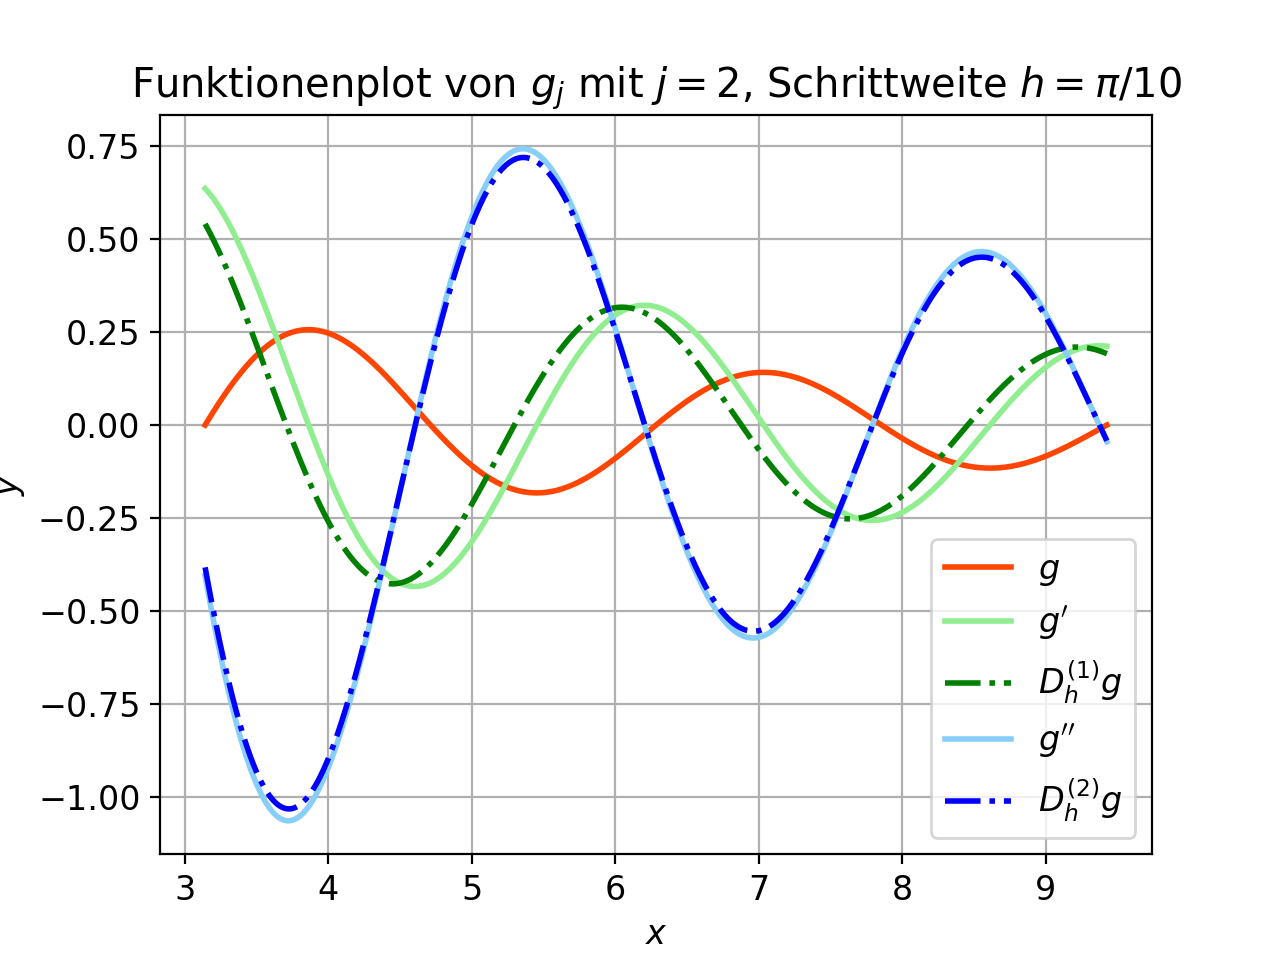
\includegraphics[width=0.42\textwidth]{Grafiken/Funktionenplot_j2_Pi_Zehntel}
    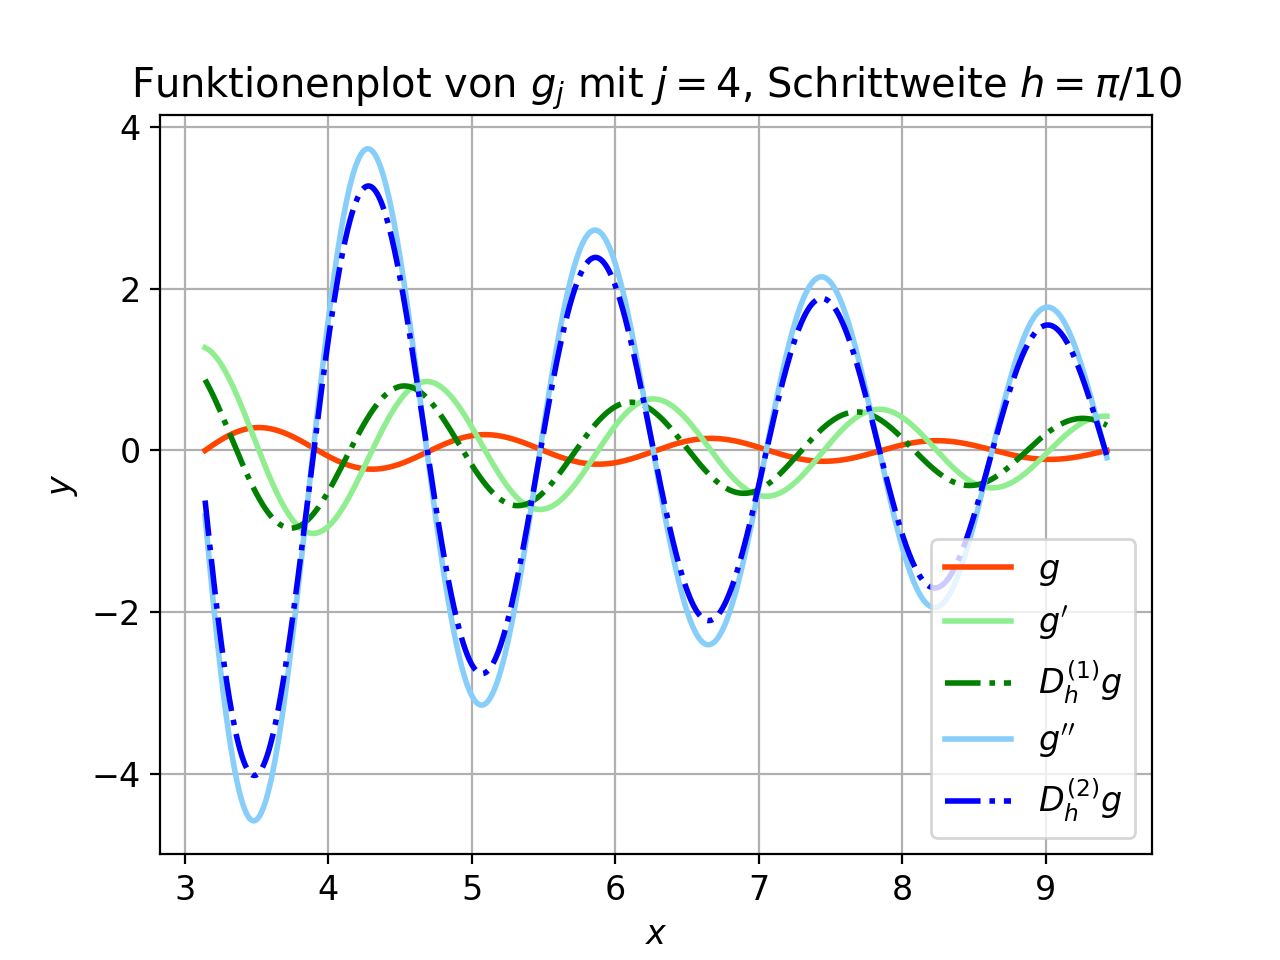
\includegraphics[width=0.42\textwidth]{Grafiken/Funktionenplot_j4_Pi_Zehntel}\\
    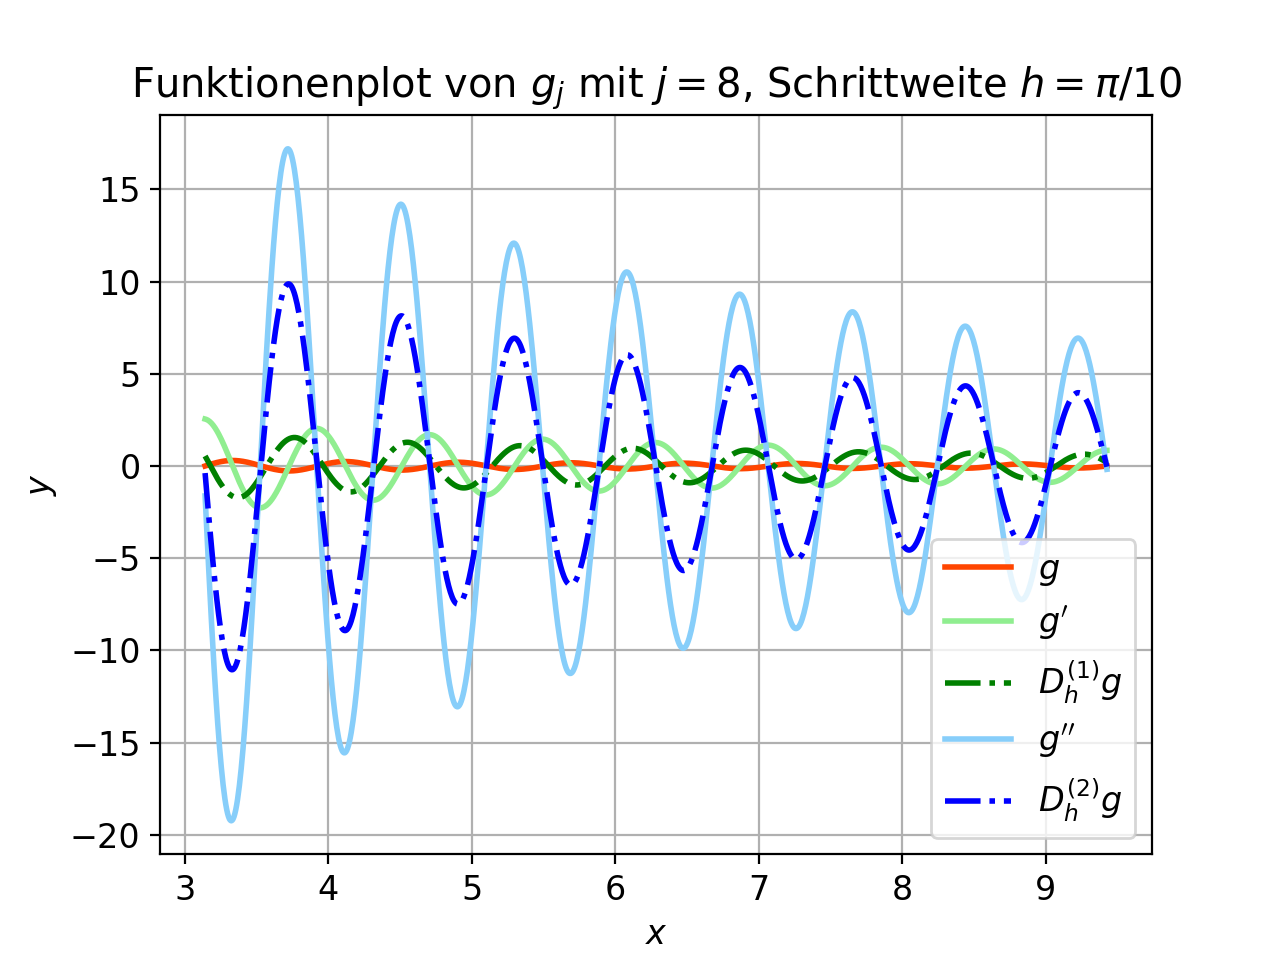
\includegraphics[width=0.42\textwidth]{Grafiken/Funktionenplot_j8_Pi_Zehntel}
    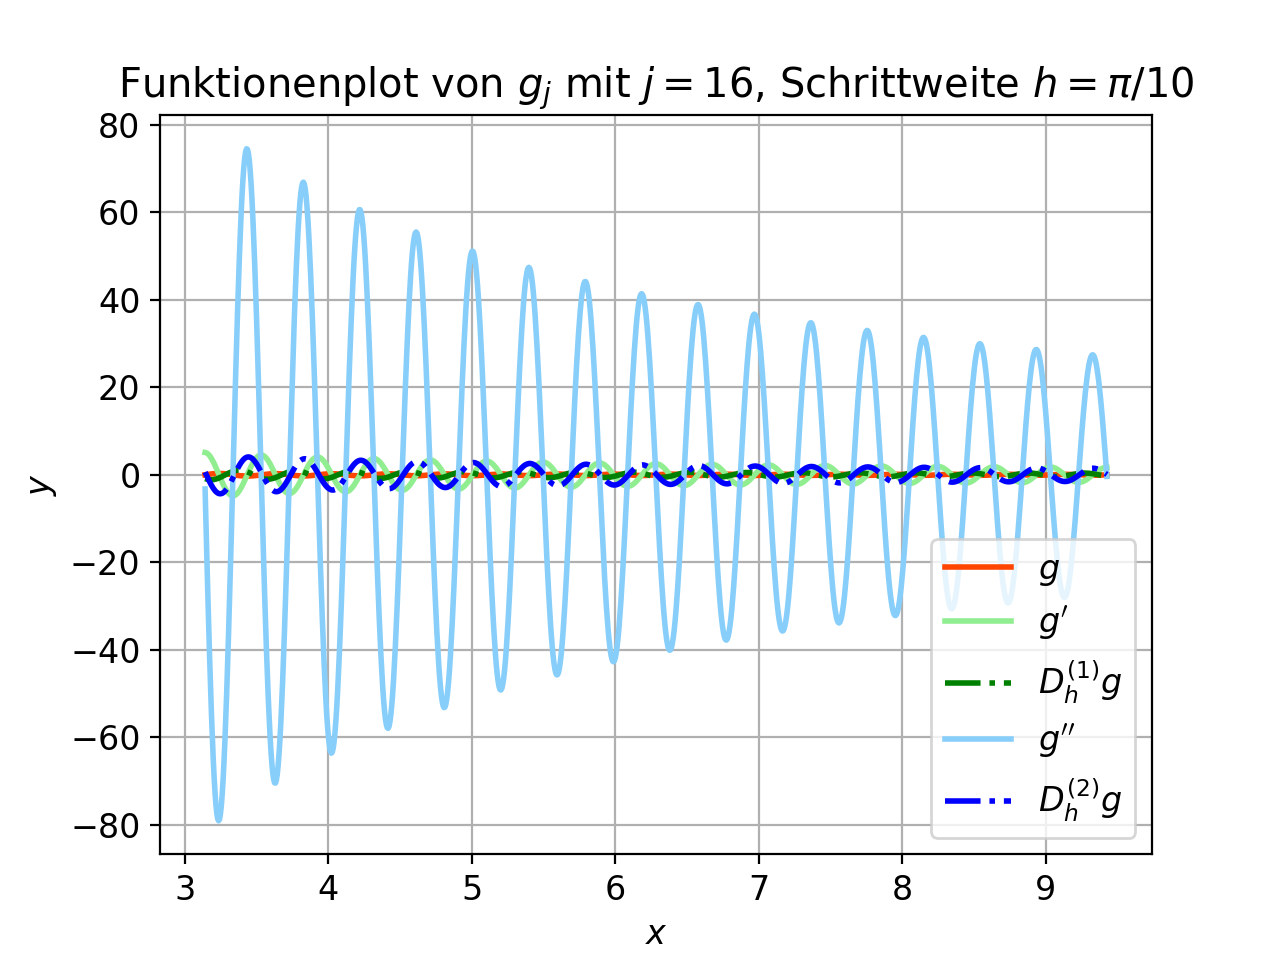
\includegraphics[width=0.42\textwidth]{Grafiken/Funktionenplot_j16_Pi_Zehntel}\\
    \vspace{-0.2cm}
    \captionof{figure}{Funktionenplots von $g_j$ für $j>1$}

    \vspace{0.5cm}
    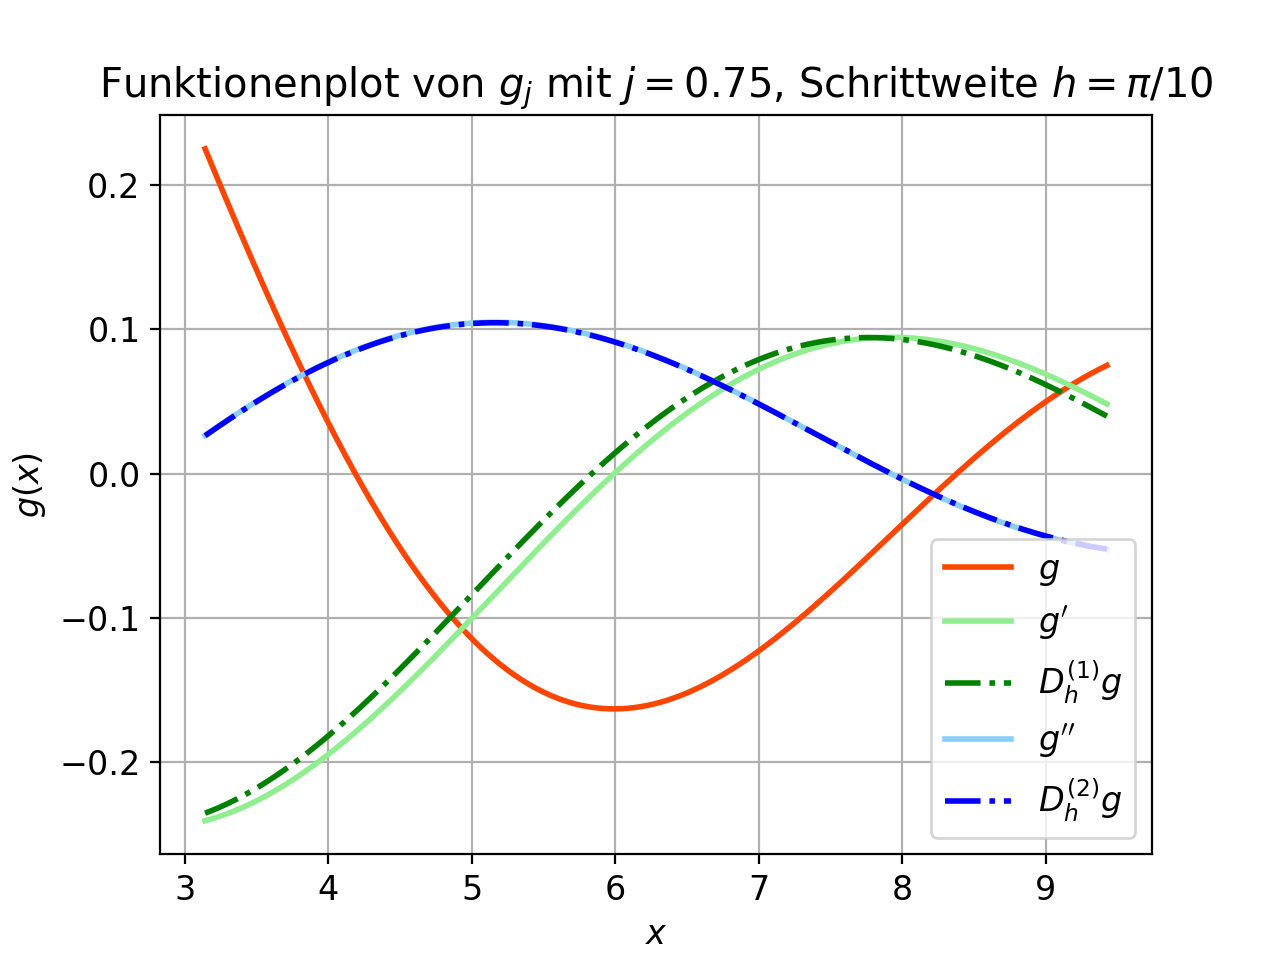
\includegraphics[width=0.42\textwidth]{Grafiken/Funktionenplot_j075_Pi_Zehntel}
    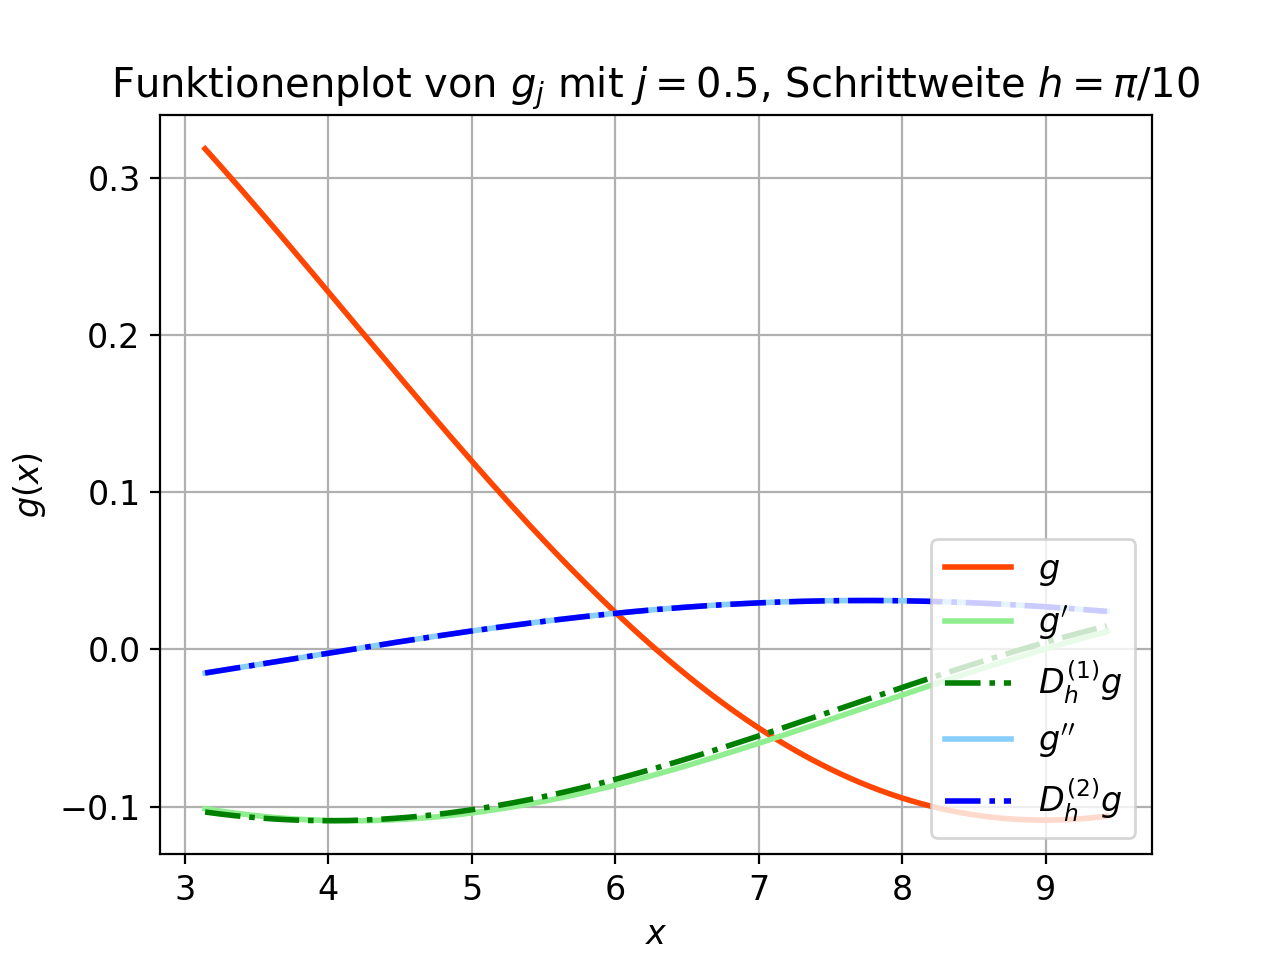
\includegraphics[width=0.42\textwidth]{Grafiken/Funktionenplot_j05_Pi_Zehntel}\\
    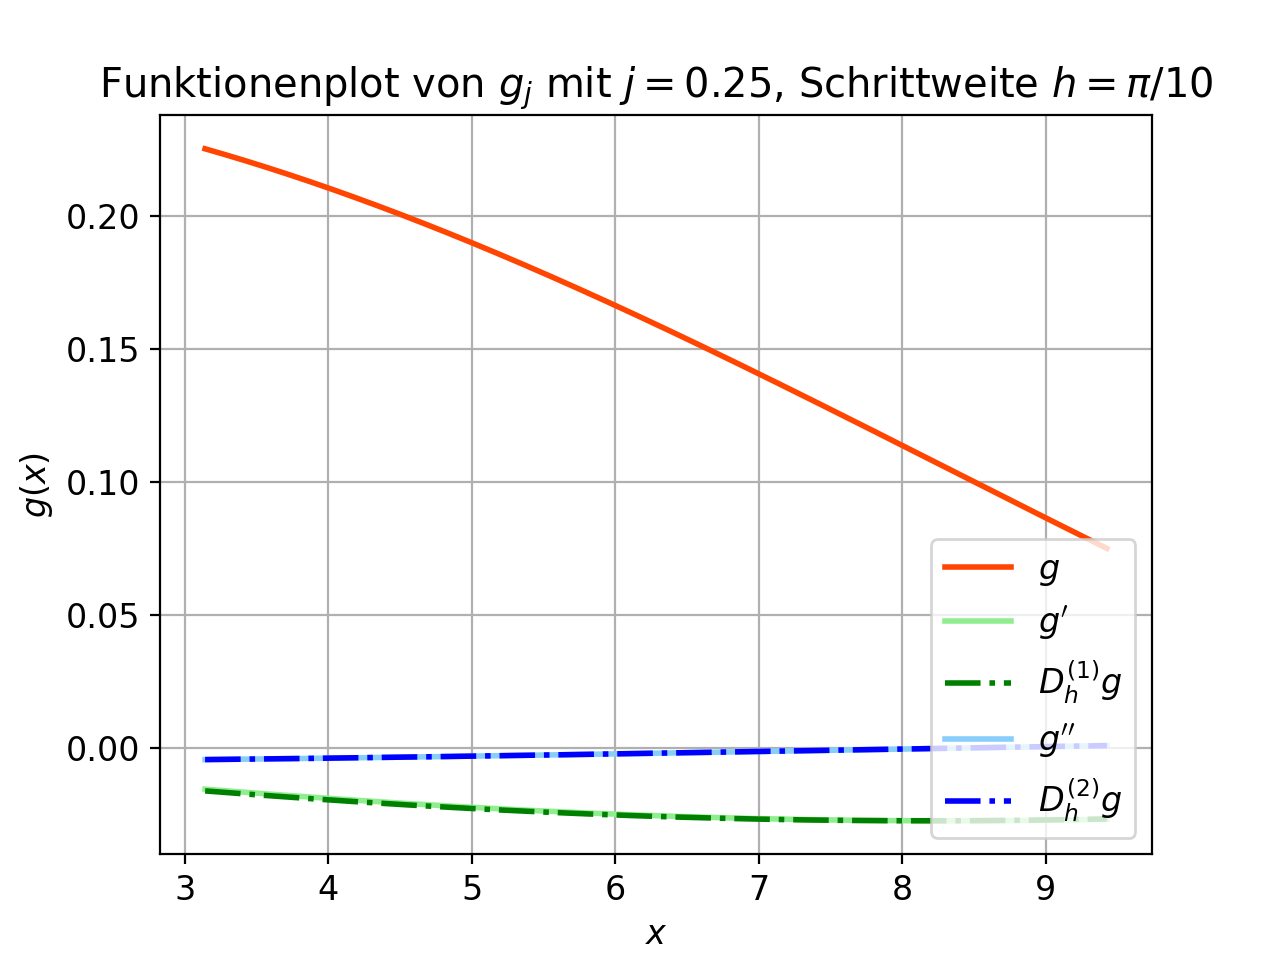
\includegraphics[width=0.42\textwidth]{Grafiken/Funktionenplot_j025_Pi_Zehntel}
    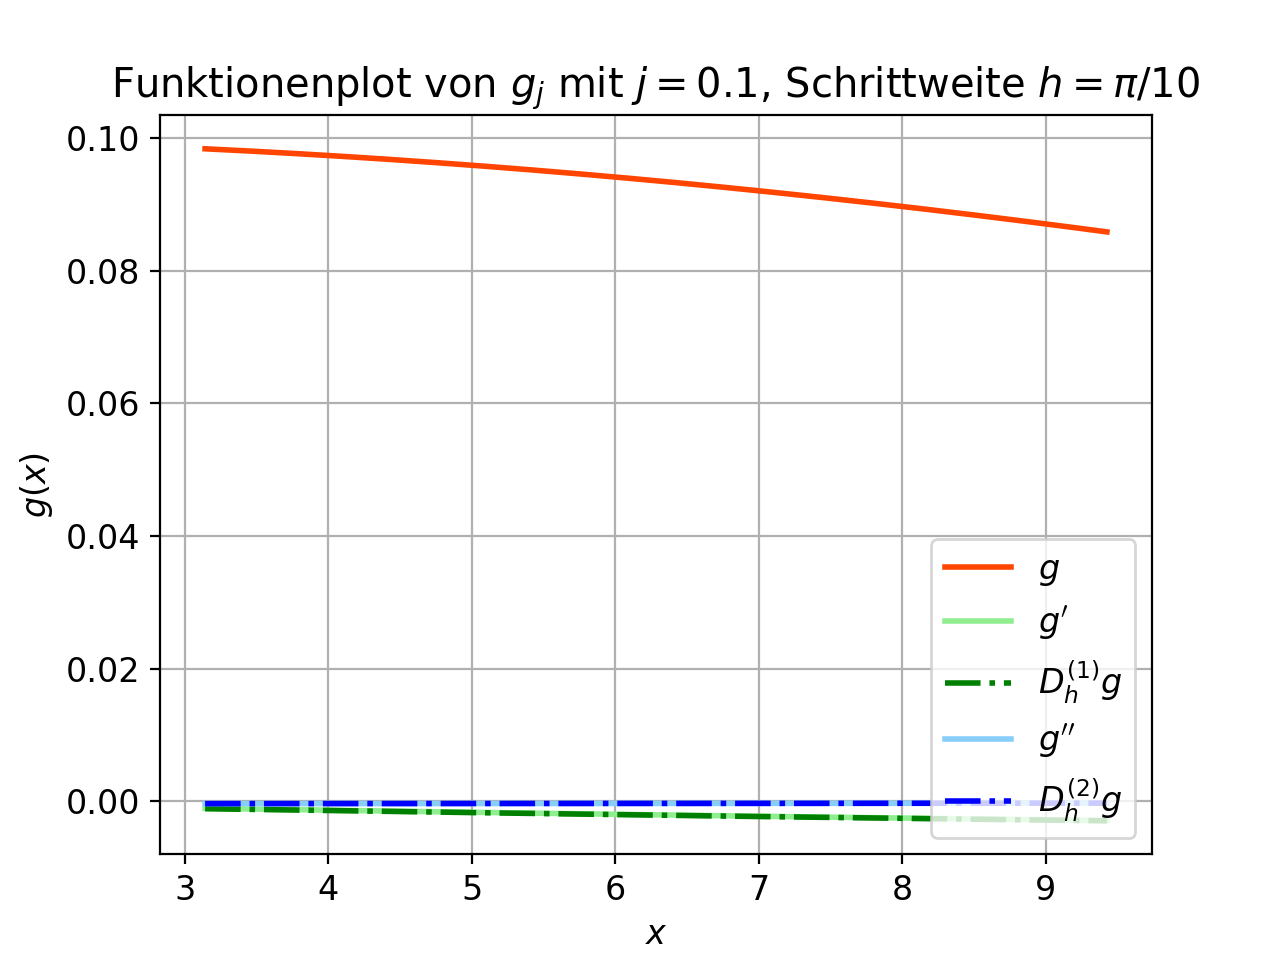
\includegraphics[width=0.42\textwidth]{Grafiken/Funktionenplot_j01_Pi_Zehntel}\\
    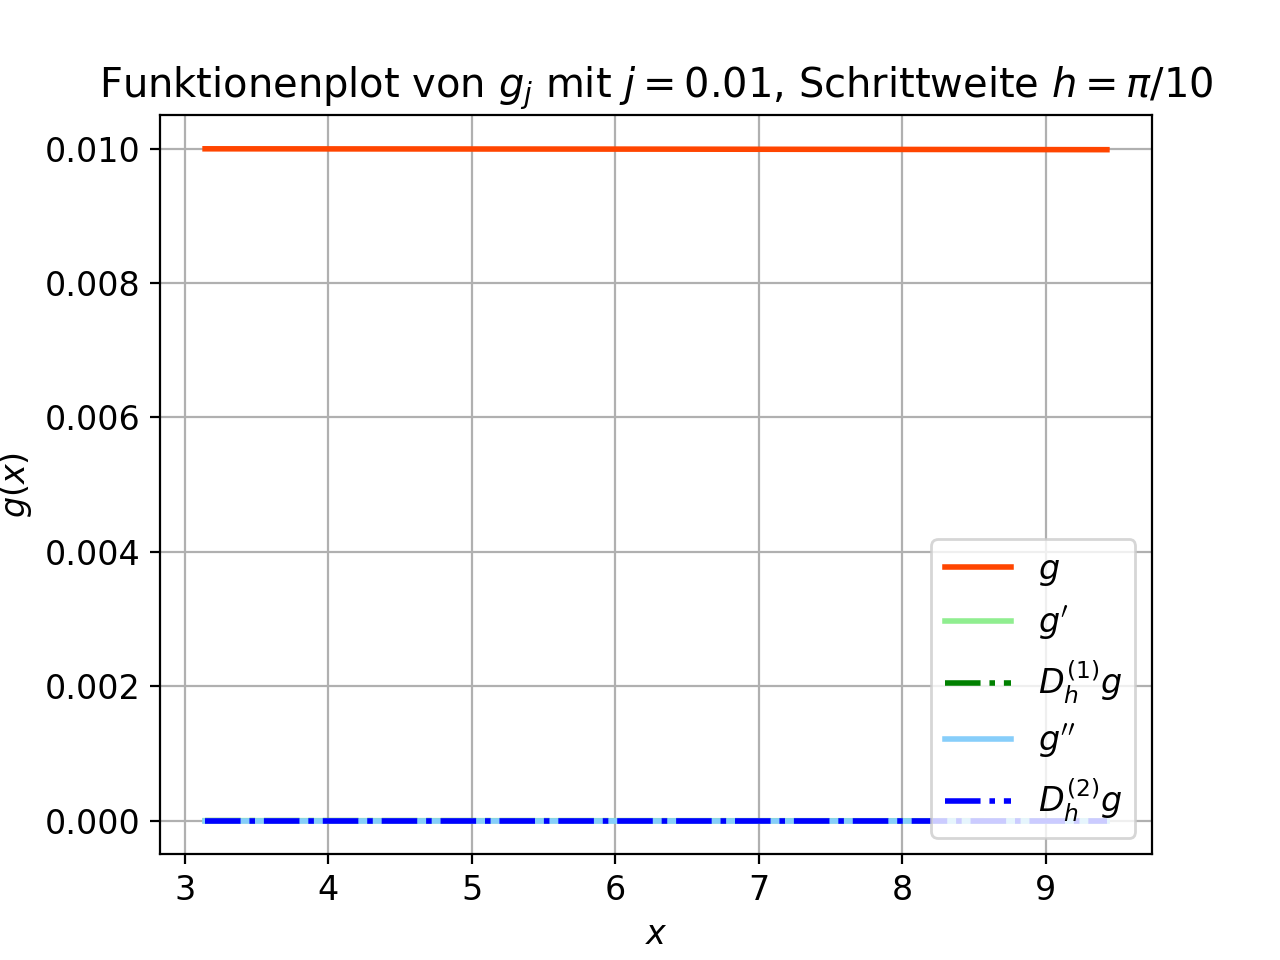
\includegraphics[width=0.42\textwidth]{Grafiken/Funktionenplot_j001_Pi_Zehntel}
    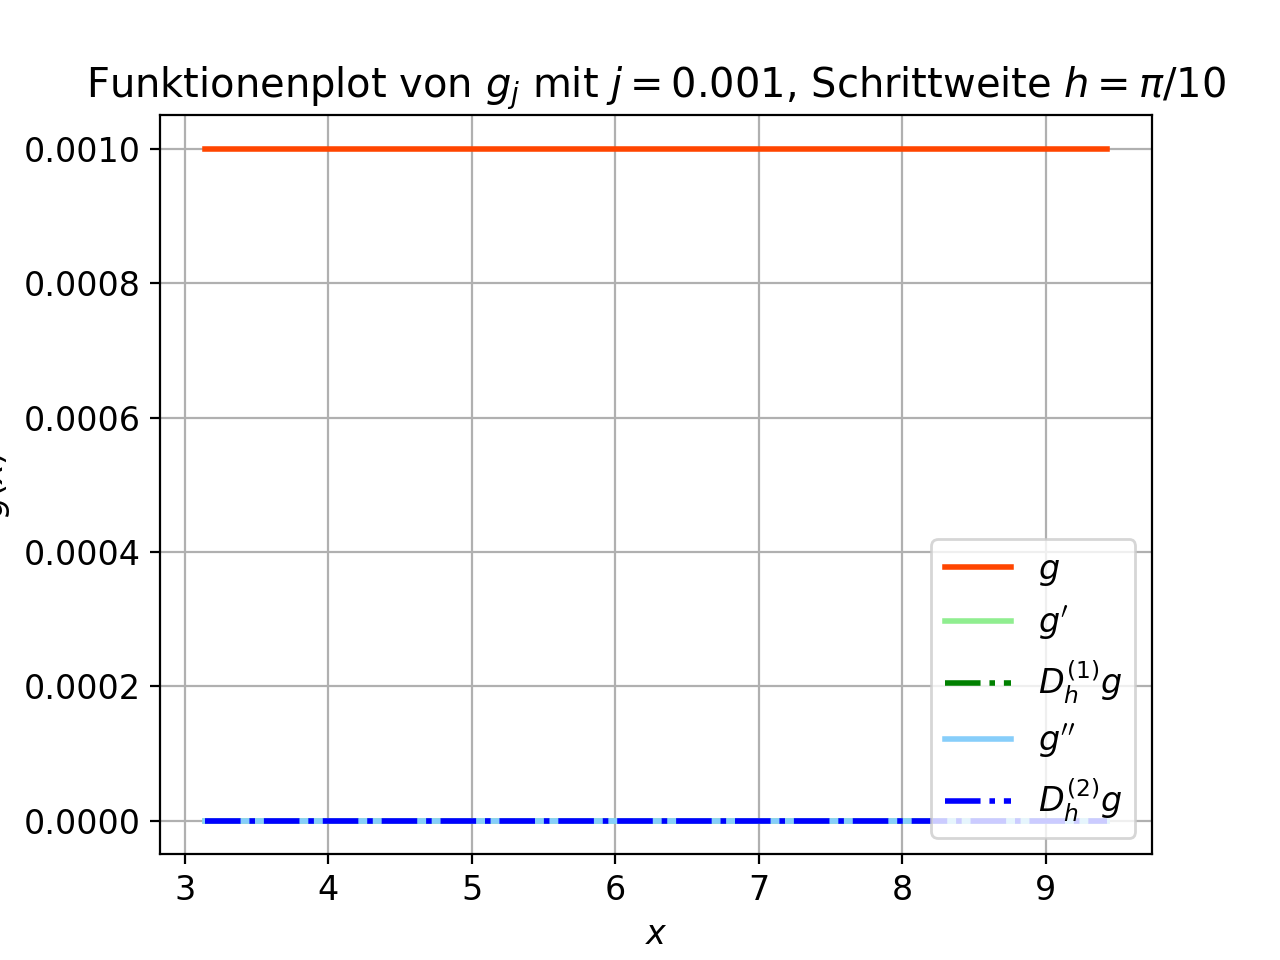
\includegraphics[width=0.42\textwidth]{Grafiken/Funktionenplot_j0001_Pi_Zehntel}\\
    \vspace{-0.2cm}
    \captionof{figure}{Funktionenplots von $g_j$ für $j<1$}

    \vspace{0.5cm}
  }

Auch bei den Fehlerplots lässt sich jeweils gegenteiliges Verhalten beobachten. Während die Größenordnung des Approximationsfehlers bei immer größere $j$'s für die dargestellten Schrittweiten zunimmt, nimmt sie bei immer kleineren $j$'s ab. Zudem verschiebt sich die Stelle, ab der der Fehler nicht weiter kleiner wird und die lineare bzw. quadratische Konvergenzgeschwindigkeit nicht mehr erkennbar ist: Bei immer größeren $j$'s verschiebt sie sich nach links, d.h. ab immer feinerem $h$. Bei immer kleineren $j$'s verschiebt sie sich nach rechts, d.h. ab immer gröberem $h$. Ebenso ist hier erkennbar, dass sich der Beginn des $h$-Intervalls, in dem die lineare bzw. quadratische Konvergenz des Verfahren sichtbar ist, nach links bzw. nach rechts verschiebt. Dieser Konvergenz-Bereich verschwindet zunehmend aus dem Blickfeld und sichtbar wird bei immer größeren $j$'s der Bereich rechts davon und bei immer kleineren $j$'s der Bereich links davon.

\vspace{0.4cm}
{
  \centering
    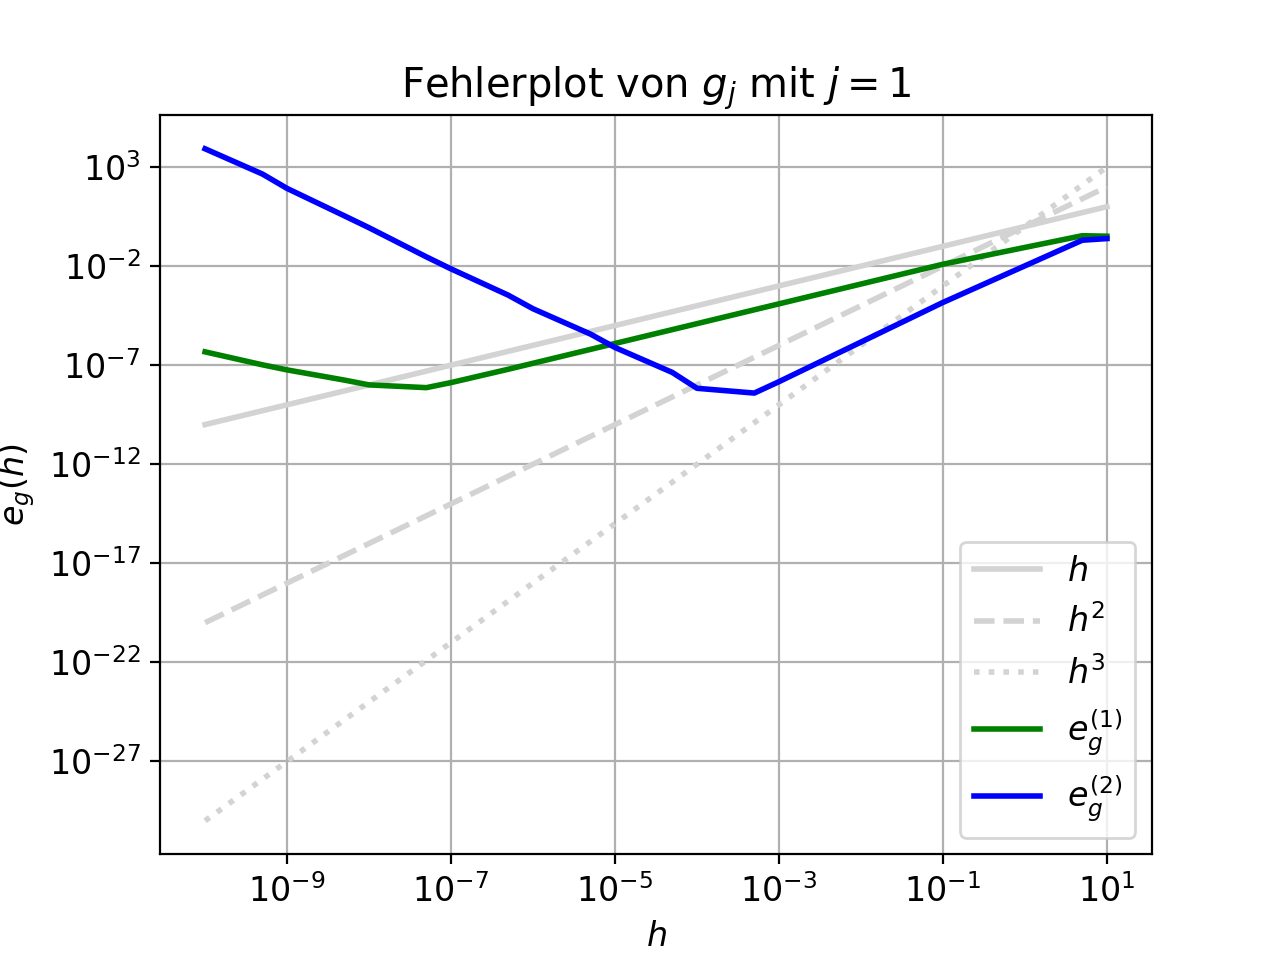
\includegraphics[width=0.45\textwidth]{Grafiken/Fehlerplot_j1}
    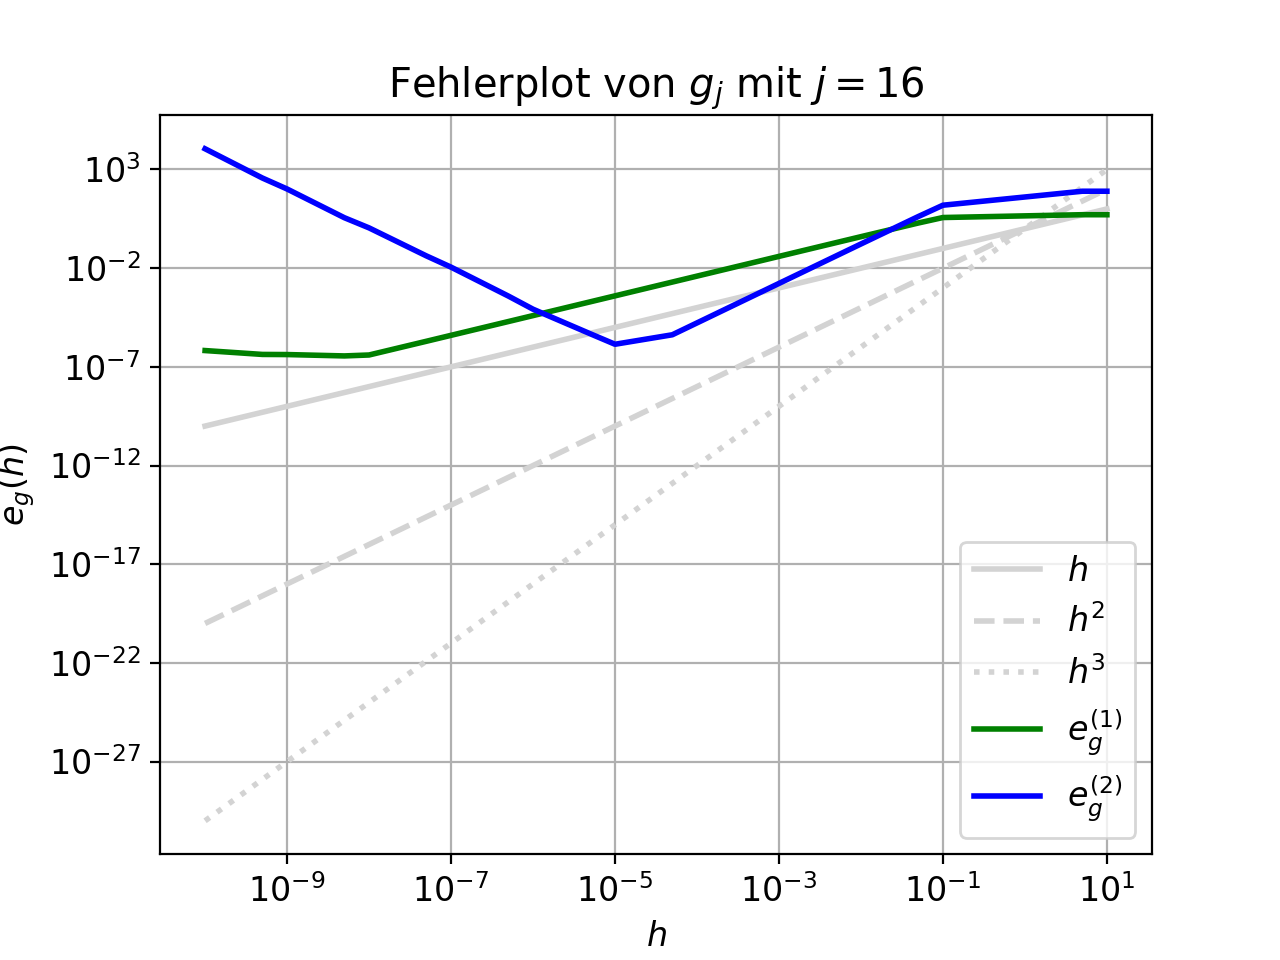
\includegraphics[width=0.45\textwidth]{Grafiken/Fehlerplot_j16}\\
    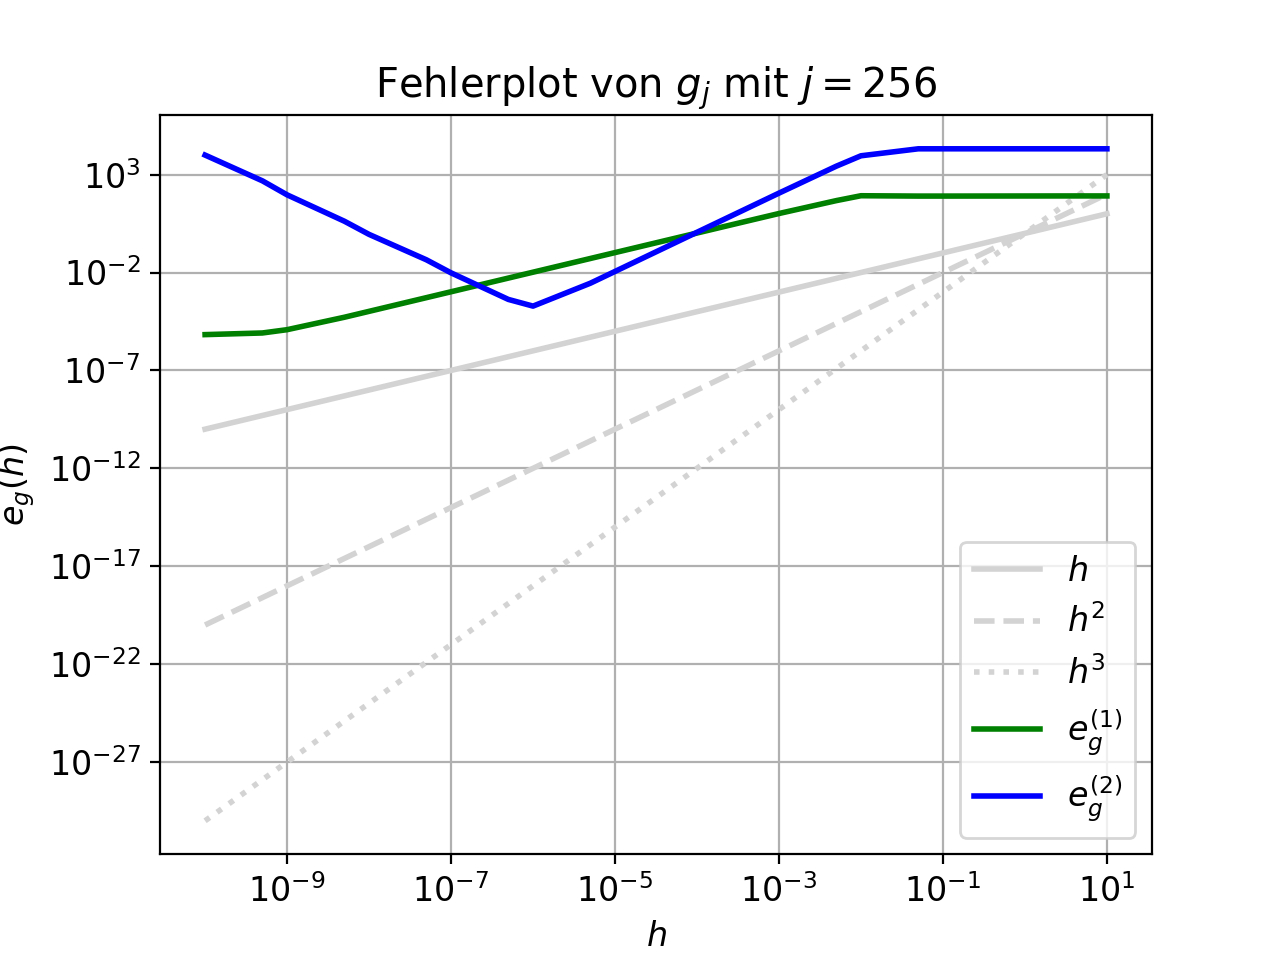
\includegraphics[width=0.45\textwidth]{Grafiken/Fehlerplot_j256}
    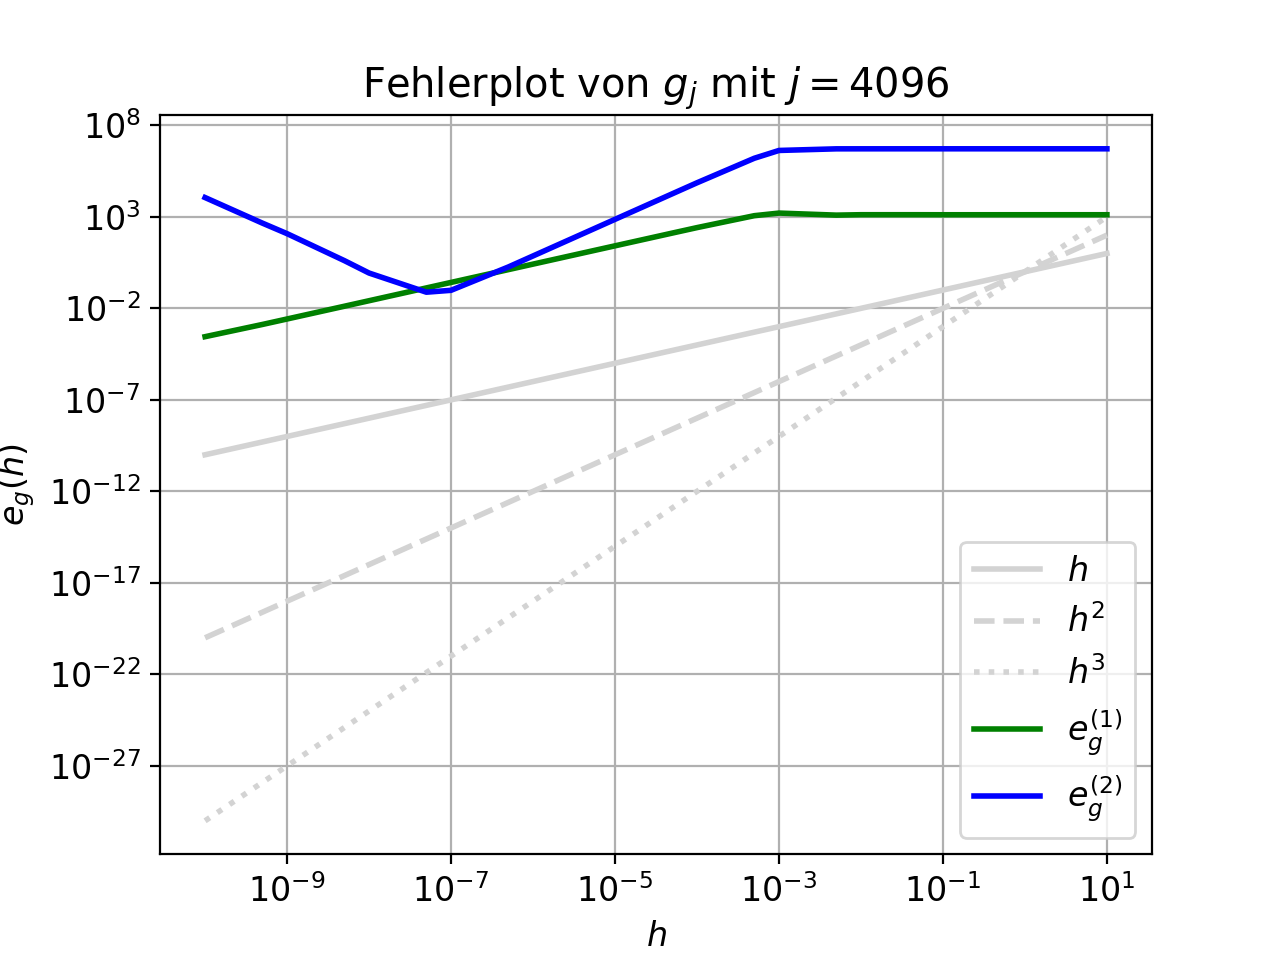
\includegraphics[width=0.45\textwidth]{Grafiken/Fehlerplot_j4096}\\
    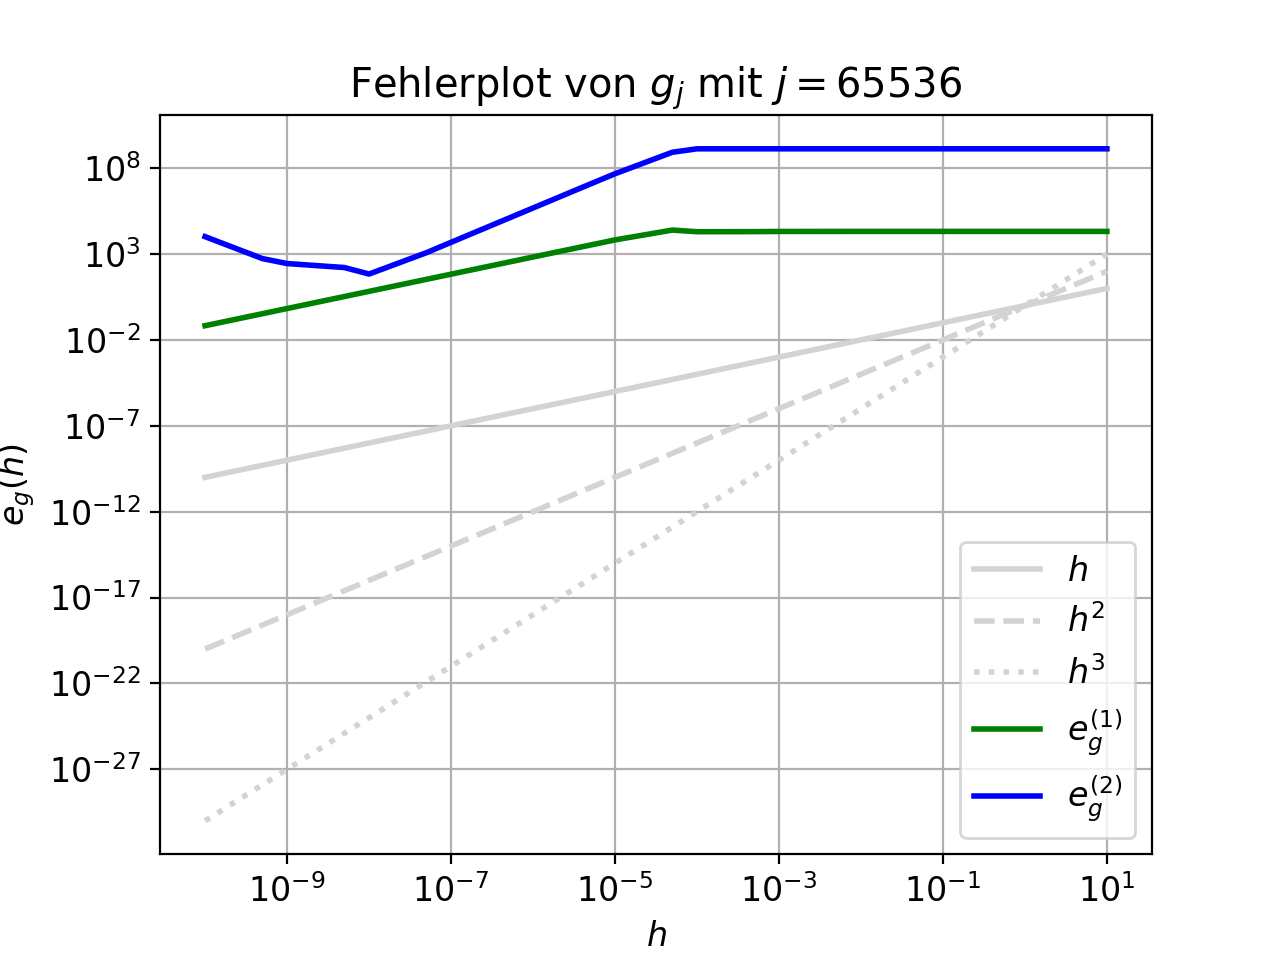
\includegraphics[width=0.45\textwidth]{Grafiken/Fehlerplot_j65536}
    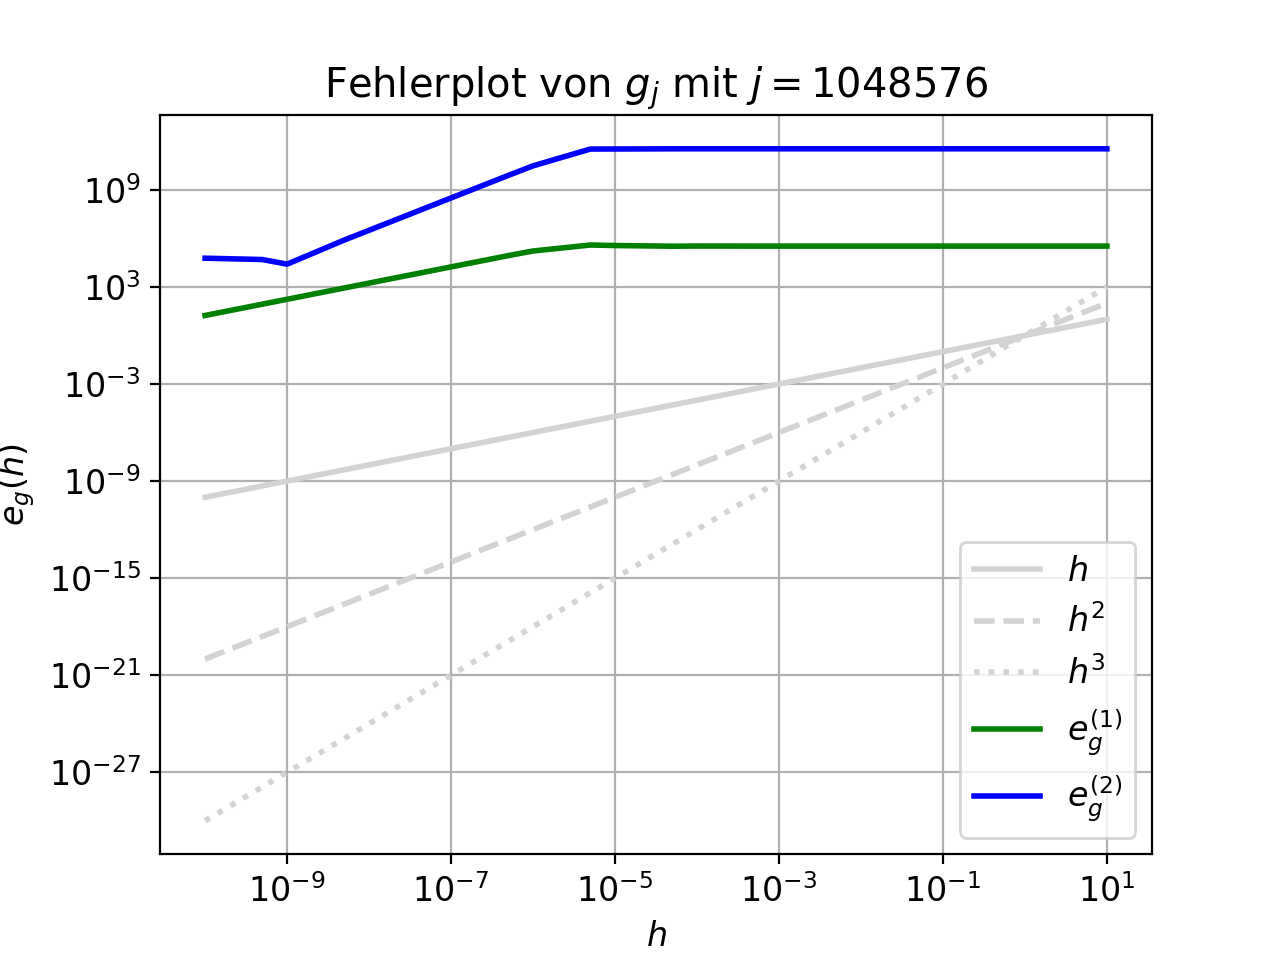
\includegraphics[width=0.45\textwidth]{Grafiken/Fehlerplot_j1048576}\\
    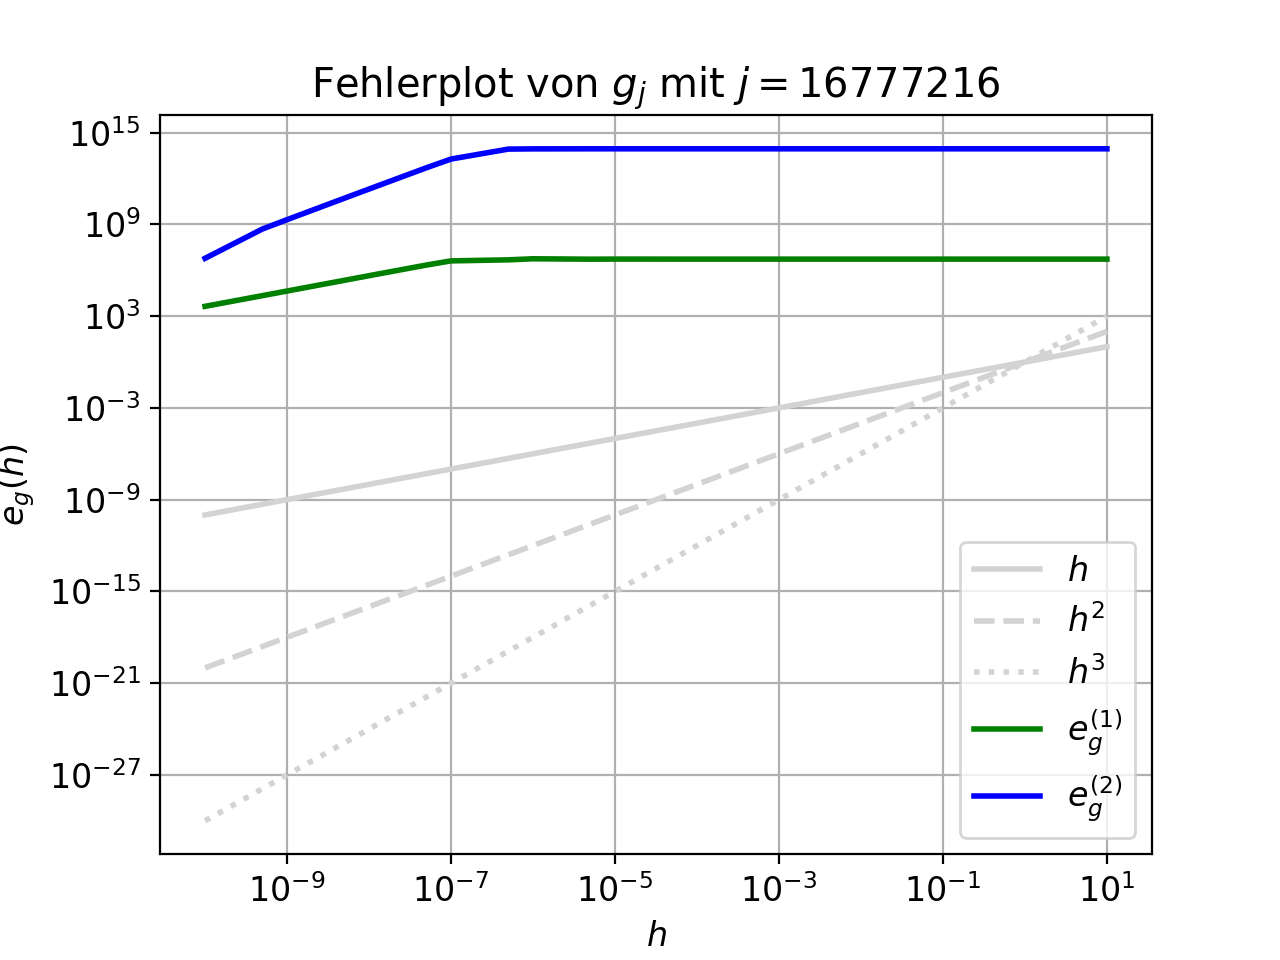
\includegraphics[width=0.45\textwidth]{Grafiken/Fehlerplot_j16777216}
    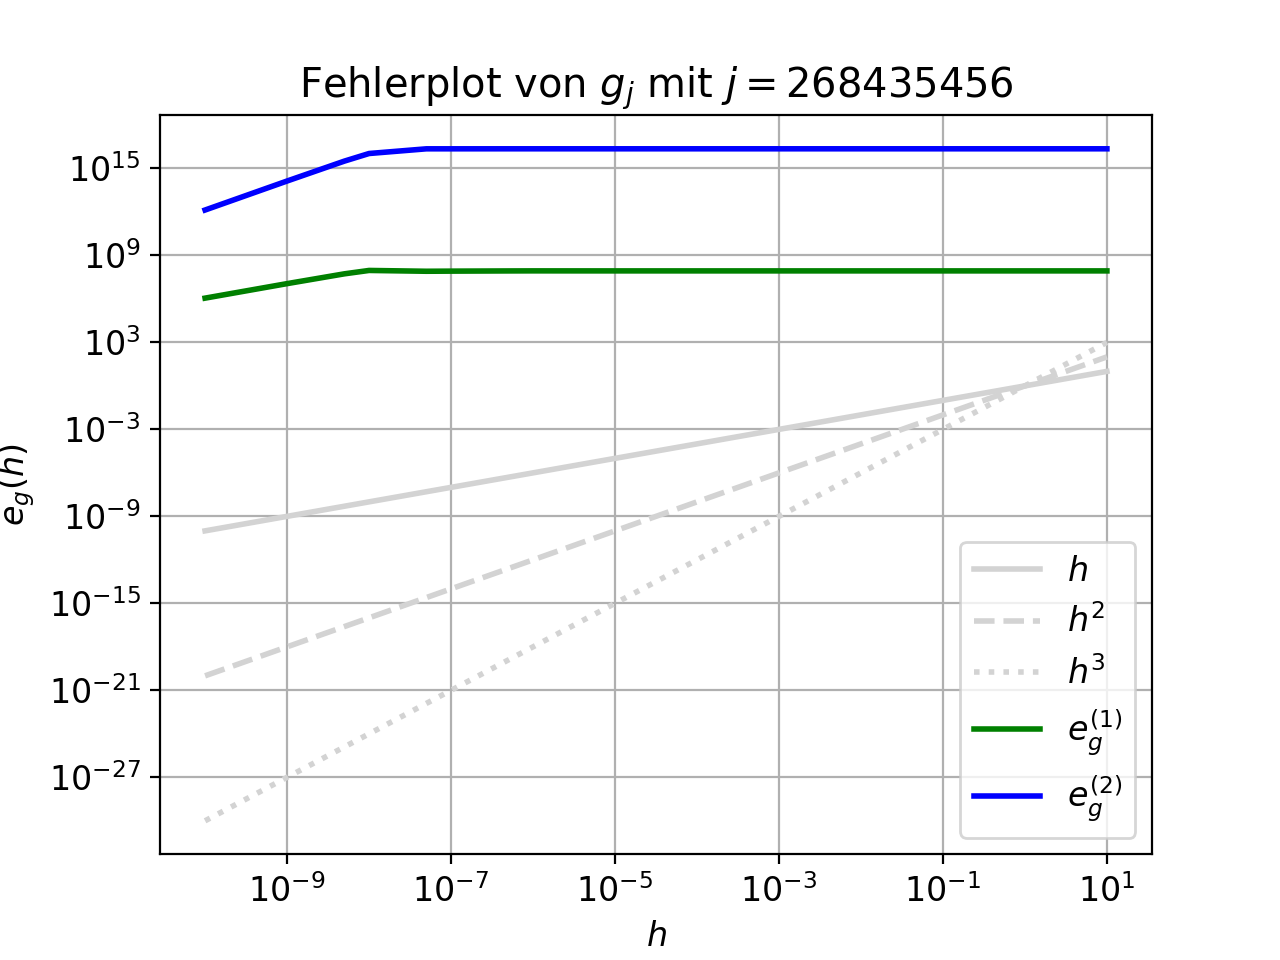
\includegraphics[width=0.45\textwidth]{Grafiken/Fehlerplot_j268435456}\\
    \vspace{-0.2cm}
    \captionof{figure}{Fehlerplots von $g_j$ für verschiedene $j>1$}

    \vspace{0.5cm}

    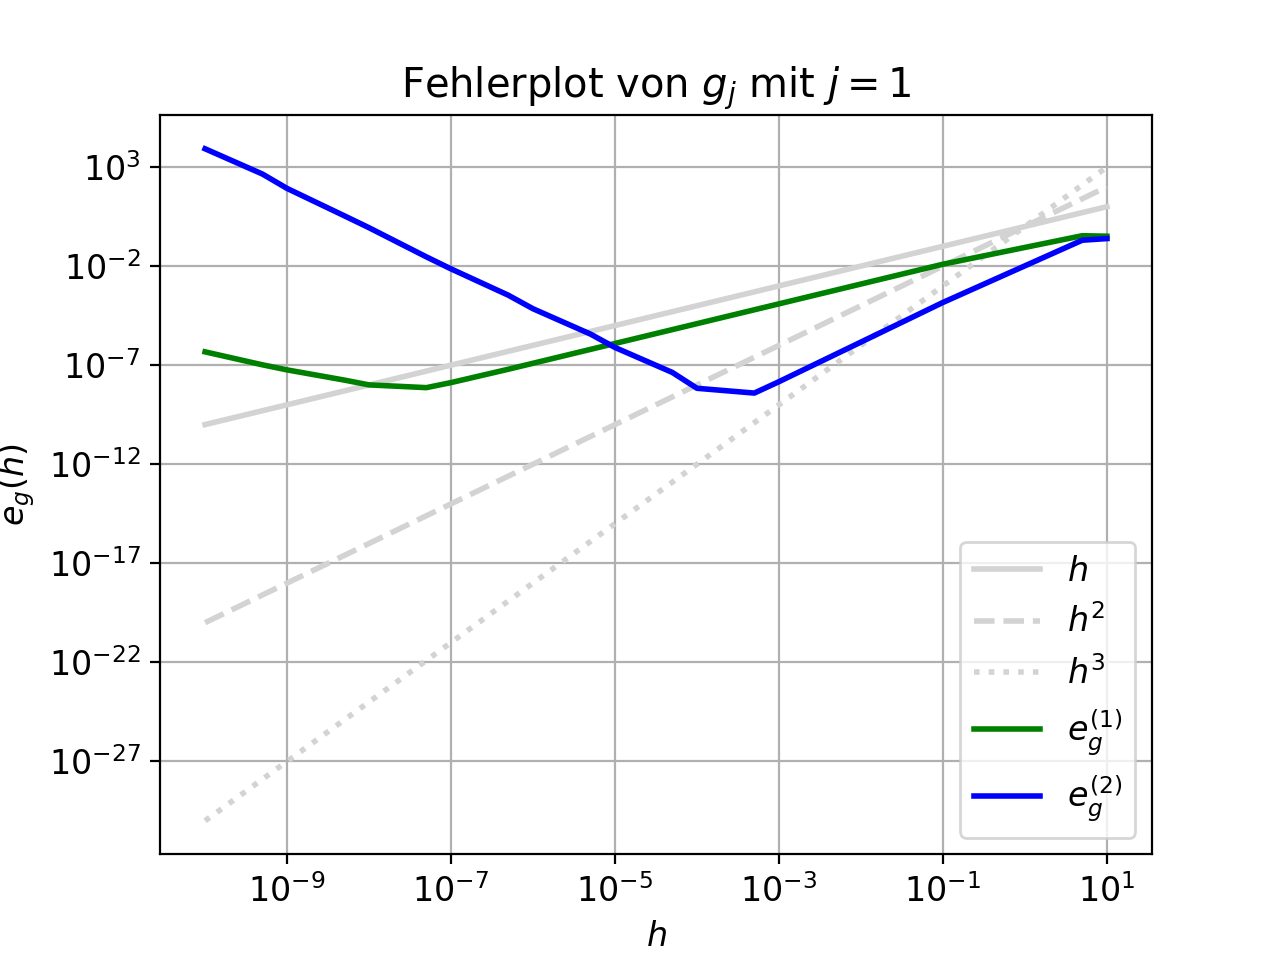
\includegraphics[width=0.45\textwidth]{Grafiken/Fehlerplot_j1}
    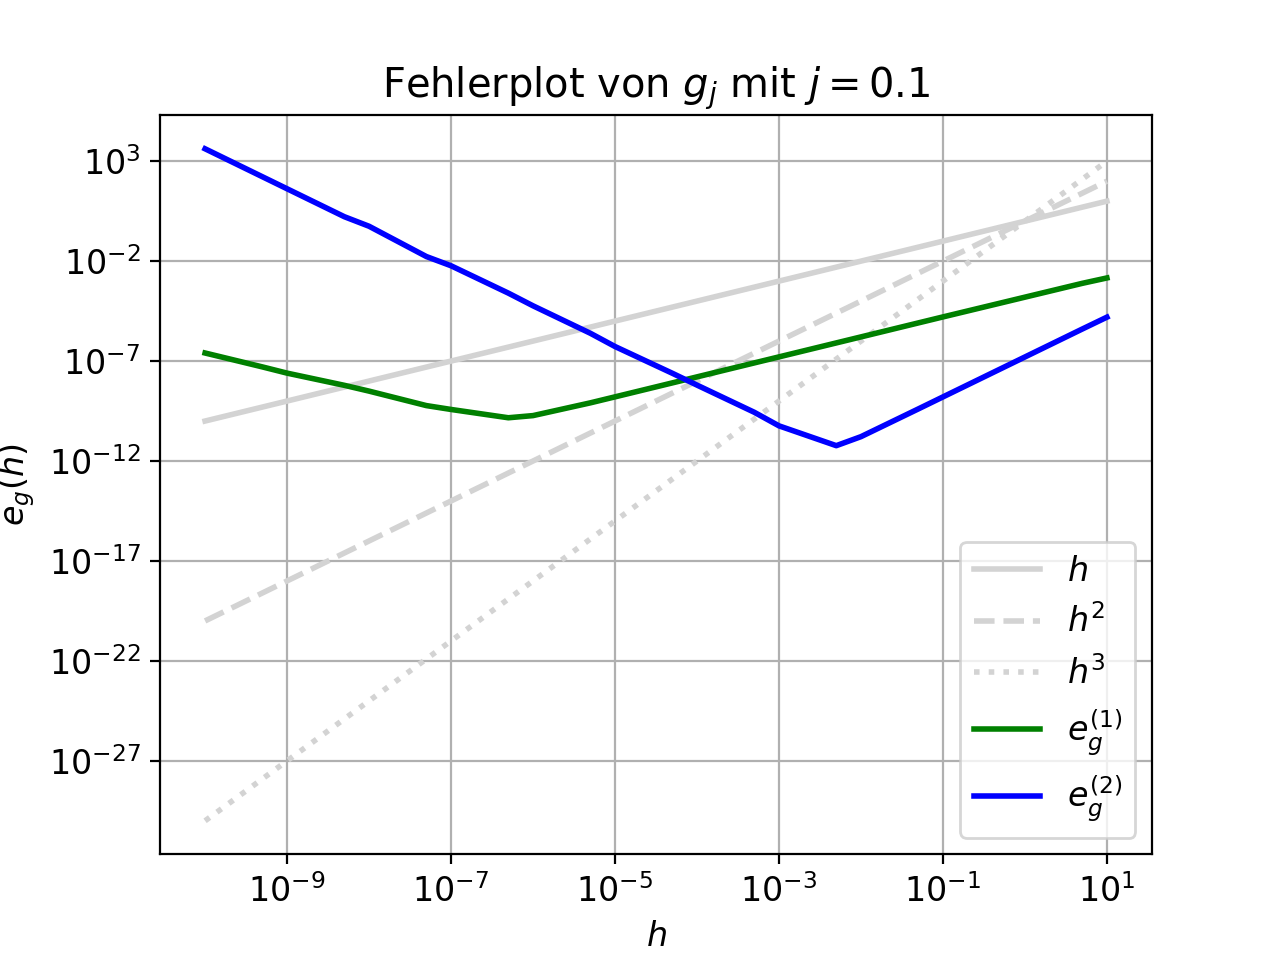
\includegraphics[width=0.45\textwidth]{Grafiken/Fehlerplot_j01}\\
    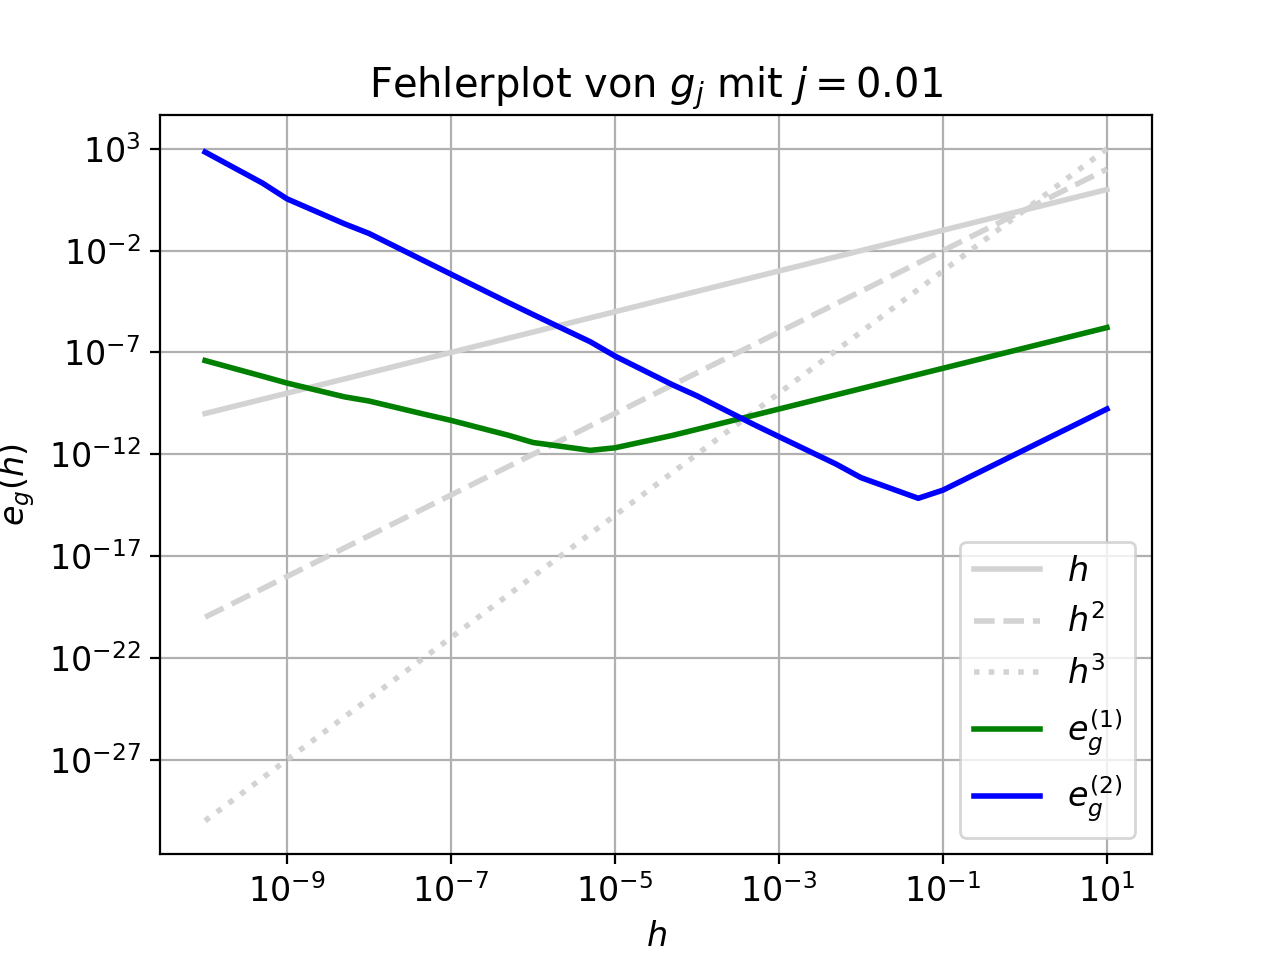
\includegraphics[width=0.45\textwidth]{Grafiken/Fehlerplot_j001}
    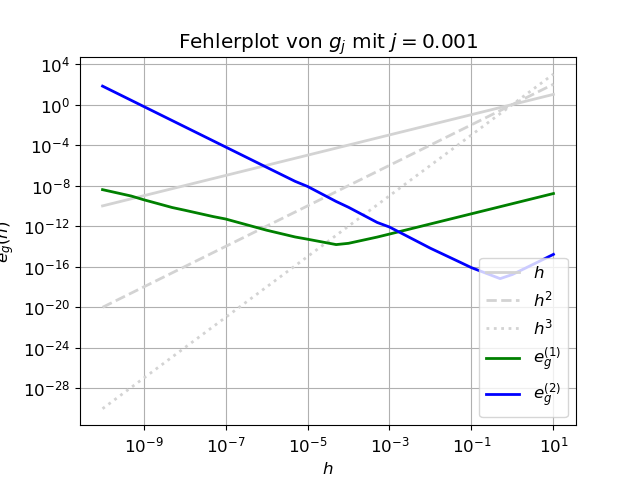
\includegraphics[width=0.45\textwidth]{Grafiken/Fehlerplot_j0001}\\
    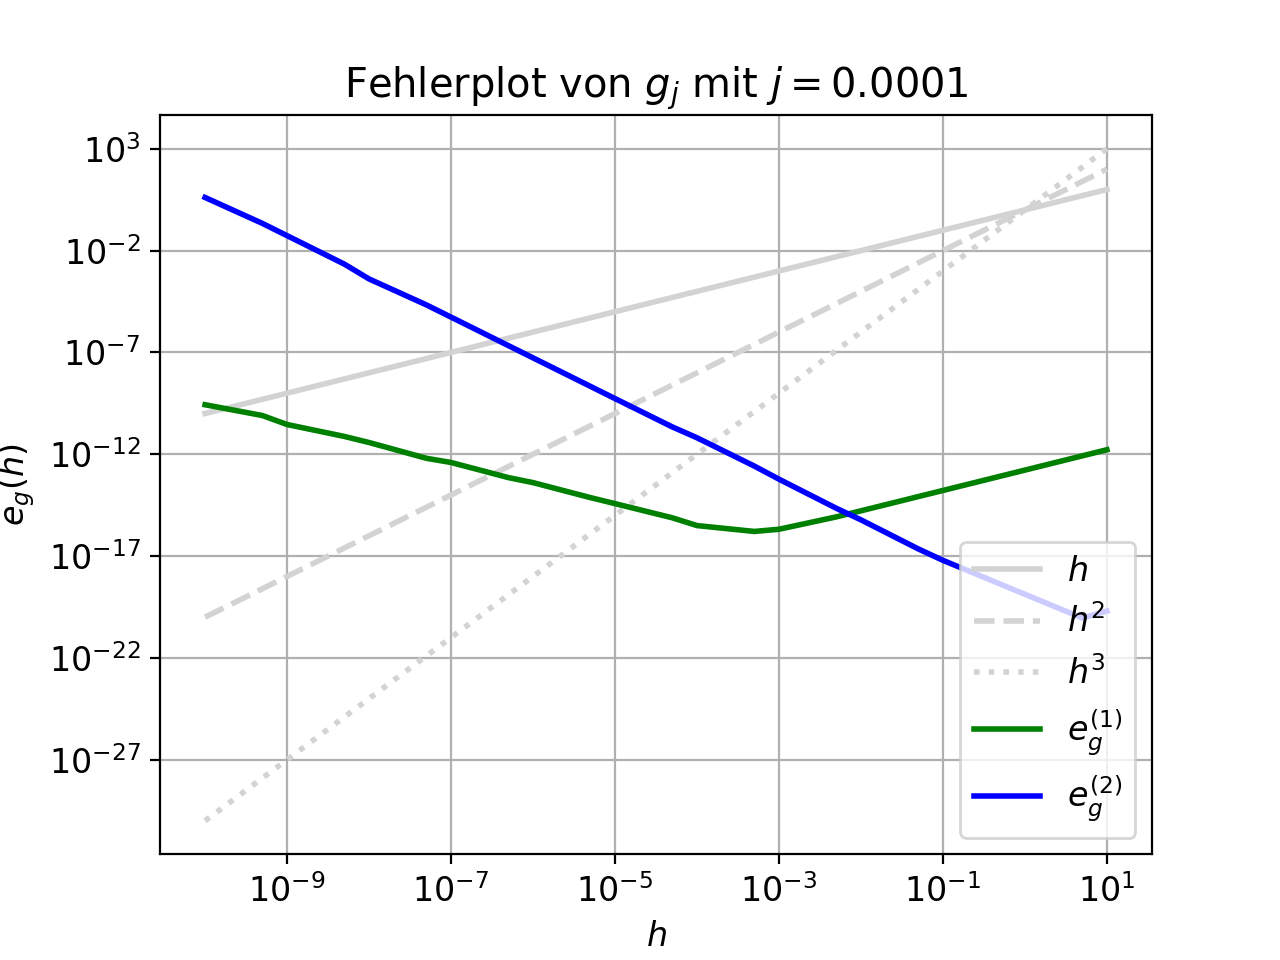
\includegraphics[width=0.45\textwidth]{Grafiken/Fehlerplot_j00001}
    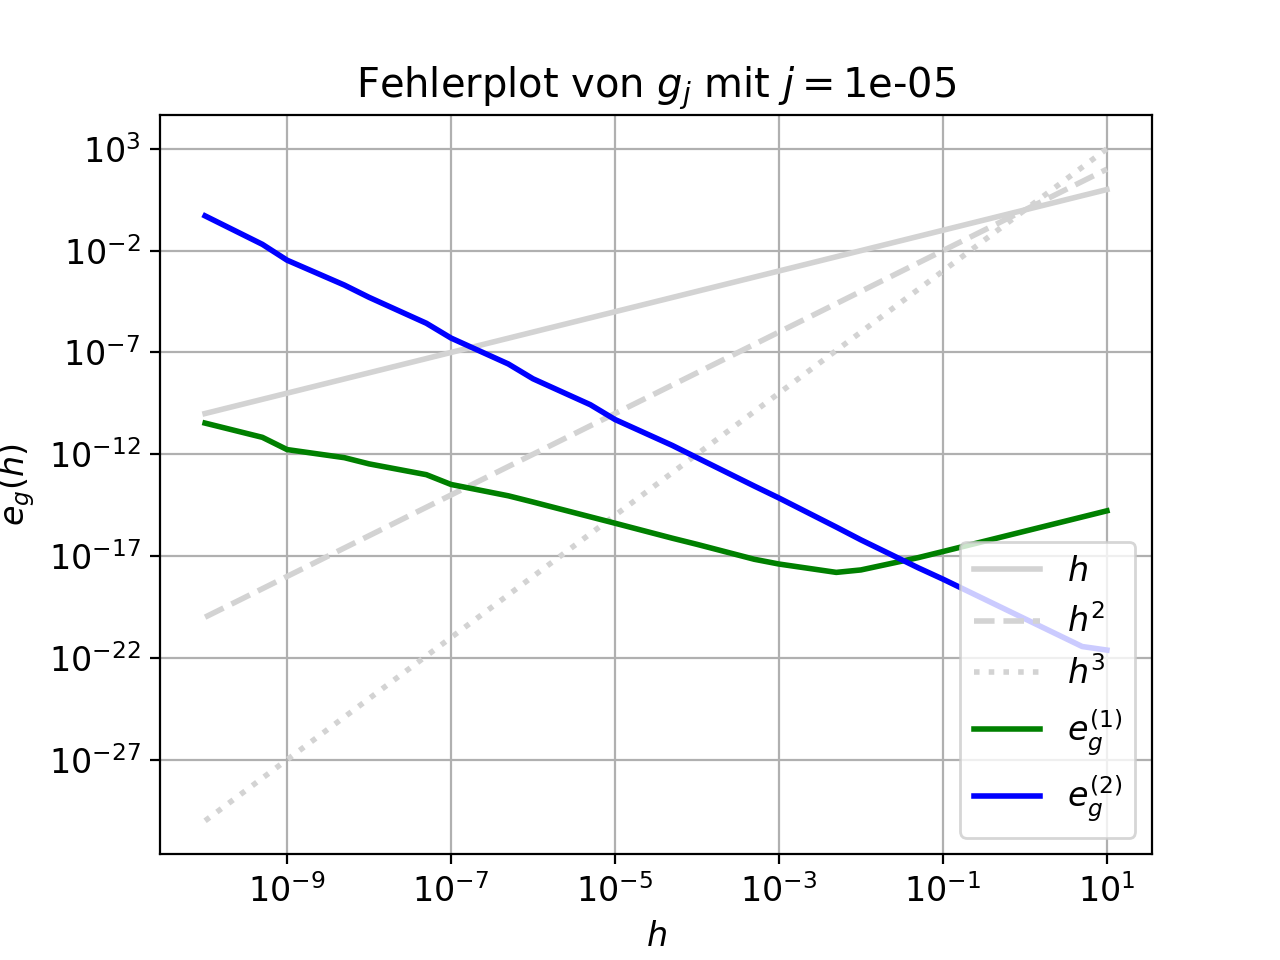
\includegraphics[width=0.45\textwidth]{Grafiken/Fehlerplot_j000001}\\
    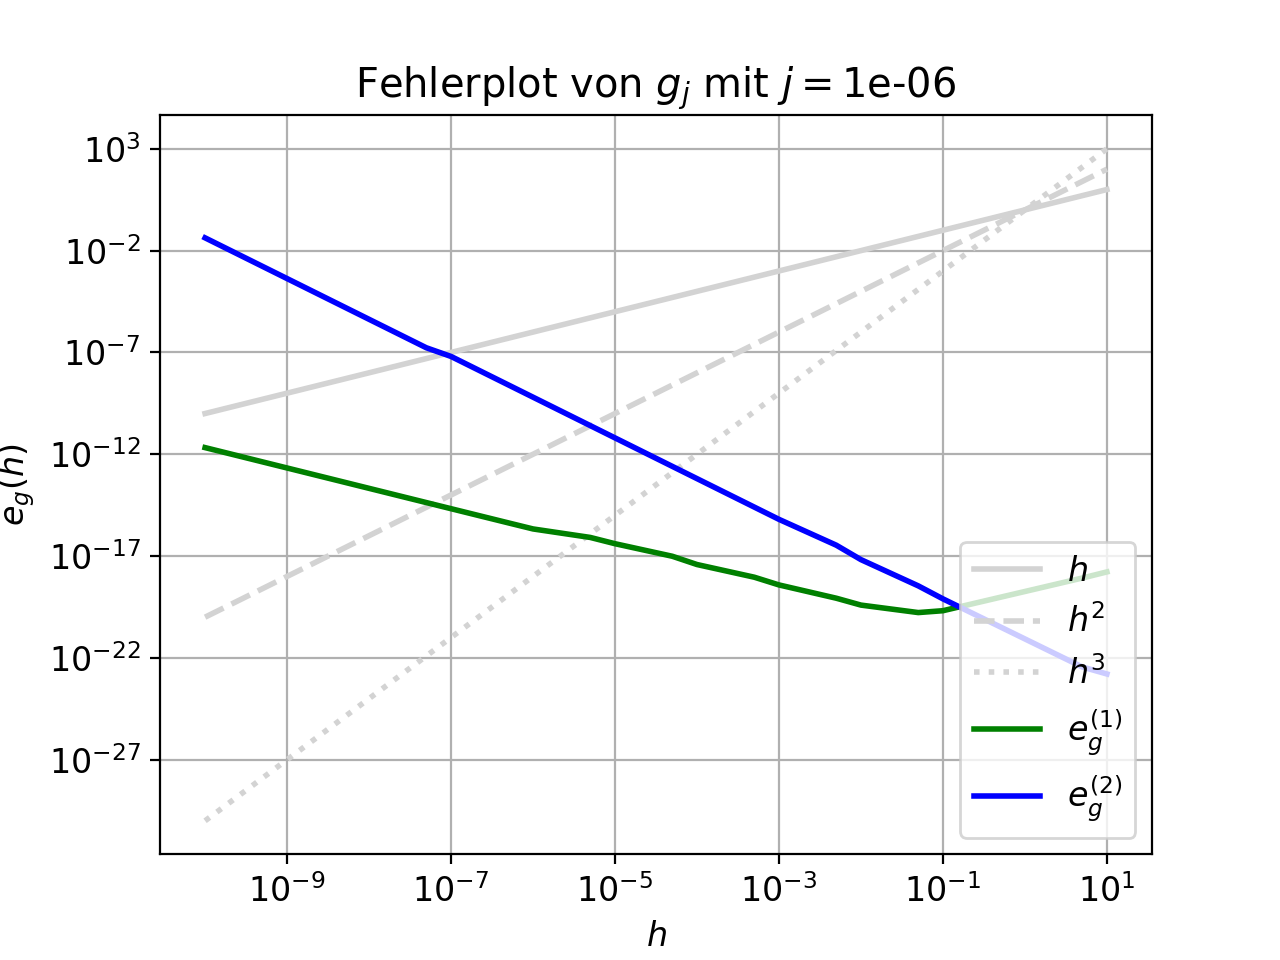
\includegraphics[width=0.45\textwidth]{Grafiken/Fehlerplot_j0000001}
    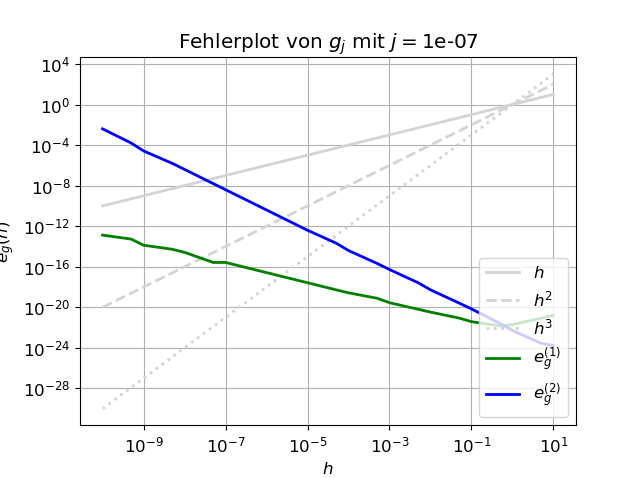
\includegraphics[width=0.45\textwidth]{Grafiken/Fehlerplot_j00000001}\\
    \vspace{-0.2cm}
    \captionof{figure}{Fehlerplots von $g_j$ für verschiedene $j<1$}
    \vspace{0.5cm}
  }

\pagebreak \section{Auswertung}
\label{sec:auswertung}
Dass die Approximation der Ableitungen der Funktion $g_1:[\pi, 3\pi] \rightarrow \mathbb{R}$ mit $g_1(x)=sin(x)/x$ für kleinere Schrittweiten $h$ immer genauer wurde, lässt sich damit erklären, dass sich die Stelle $x+h$ beim Verkleinern der Schrittweite $h$ immer weiter der zu untersuchenden Stelle $x$ nähert.
Die Sekantensteigung kommt also der exakten Tangentensteigung immer näher.
Dass sich die zweite finite Differenz dabei schneller der analytischen zweiten Ableitung als die erste finite Differenz der analytischen ersten Ableitung nähert, ist mittels der oben gemachten theoretischen Überlegungen darauf zurückzuführen, dass der Fehler der ersten finiten Differenz linear von $h$ abhängt, der Fehler der zweiten finiten Differenz allerdings sogar quadratisch von $h$ abhängt.
Mit Wahl eines kleinen $h$'s ($h<1$) konvergiert die zweite finite Differenz also schneller gegen die analytische Ableitung. \\
Dass es keinen Vorteil bringt, wenn man die Schrittweite $h$ beliebig weit verkleinert, zeigte der Fehlerplot von $g_1$. Ab sehr kleinen $h$-Werten, brach die lineare bzw. quadratische Konvergenz ab, der maximale absolute Fehler wurde wieder größer.
Dieser Umstand ist der eingangs erwähnten Auslöschung geschuldet, die immer dann auftritt, wenn zwei etwa gleich große Zahlen subtrahiert werden.
Rechnet der Computer also mit der gegebenen Formel $(D_h^{(1)}g_1)(x) = \frac{g_1(x+h)-g_1(x)}{h}$ die erste finite Differenz aus und liegt $g_1(x+h)$ genügend nah an $g_1(x)$, dann reicht die Genauigkeit der Maschine und ihrer Zahlen nicht mehr aus, um die Differenz zwischen beiden gut zu berechnen. Die Genauigkeit der Rechnung und damit unserer Approximation sinkt wieder.
Auf denselben Auslöschungseffekt trifft man auch bei der Formel $(D_h^{(2)}g_1)(x) = \frac{g_1(x+h)-2g_1(x)+g_1(x-h)}{h^2}$, mit der man die zweite finite Differenz berechnet.
Aufgrund der zweifachen Division von $h$ wächst der Fehler hier quadratisch wieder an, während er bei der ersten finiten Differenz nur linear wieder anwächst. \\
 \\
In weiterführenden Experimenten haben wir die modifizierten Funktionen $g_j:[\pi, 3\pi] \rightarrow \mathbb{R}$ mit $g_j(x) = sin(j x)/x$ betrachtet. Zwei Faktoren sind maßgeblich für das beobachtete Verschieben des $h$-Bereiches, in dem die lineare bzw. quadratische Konvergenz erkennbar ist: Die Änderungsrate der Funktion auf dem untersuchten Intervall und die Größenordnung der mitspielenden Zahlen. \\
Wie man bei immer größeren $j$'s am Stauchen des Graphen in $x$-Richtung erkennen kann, nimmt die Frequenz der Funktion zu und damit auch die Änderung auf dem untersuchten Intervall (das wir beibehalten). Die Änderung der Steigung (1. Ableitung) wird immer stärker. Deswegen benötigt man für immer größere $j$'s eine feinere Schrittweite, damit eine gute Approximation gelingt. Gleiches gilt für die Krümmung des Graphen. Mehr Änderung in der ersten Ableitung von $g_j$ bewirkt auch mehr Änderung in der zweiten Ableitung. Ebenso produzieren die immer größeren Zahlen immer größere Fehler. Das Verfahren ist für die modifizierten Funktionen immer angreifbarer. Und auch nach dem "`optimalen"' $h$ muss man länger suchen. Durch die höhere Größenordnung der vom Computer zu behandelten Zahlen tritt der oben angesprochene Auslöschungseffekt erst später auf. Das mag auf den ersten Blick positiv erscheinen, aber es bedeutet auch, dass man die Schrittweite für eine möglichst genaue Approximation ebenso sehr sehr stark verringern muss, was wiederum zum einem maschinenbedingt eine untere Grenze hat und zum anderen in der Praxis mit sehr viel Aufwand verbunden ist. Insgesamt kommt es also zum Verschieben des Konvergenz-Bereiches nach links. \\
Für immer kleinere $j$'s ist das Szenario genau umgekehrt. Das Strecken des Graphen in $x$-Richtung bedeutet eine Abnahme der Frequenz und damit auch weniger Änderung auf dem betrachteten Intervall. Da die Änderung der Steigung (erste Ableitung) immer geringer wird, genügt für eine gute Approximation eine gröbere Schrittweite aus. Und auch hier gilt: \textit{more is more} oder eher \textit{less is less}. Weniger Änderung in der ersten Ableitung von $g_j$ verursacht auch weniger Änderung in der zweiten Ableitung. Da es nicht mehr viel zu tun gibt, funktioniert das Verfahren für kleinere $j$'s immer besser. Und auch hier gilt analog: Die durch die immer kleineren $j$'s kleiner werdenden Zahlen bewirken auch eine Abnahme der Größenordnung des maximalen absoluten Fehlers. Die Auslöschung setzt früher ein, das "`optimale"' $h$ ist günstig früher zu finden. Unterm Strich wird der $h$-Bereich, in dem die Konvergenz des Verfahrens erkennbar ist, nach rechts verschoben. \\

\pagebreak \section{Zusammenfassung und Ausblick}
\label{sec:zusammenfassung}
Die finiten Differenzen stellen überschaubare und leicht anwendbare Formeln bereit, um die Ableitungen einer Funktion zu approximieren.
Durch die lineare bis quadratische Konvergenz können hier mit nicht allzu großem Aufwand unter Umständen sehr genaue Näherungen geliefert werden.
Die Schwierigkeit besteht allerdings darin, einen Wert für die Schrittweite $h$ zu finden, der weder zu groß ist, um eine gute, sprich eine relativ genaue Approximation zu liefern, noch so klein, dass es durch den maschinenbedingten Auslöschungseffekt zu Fehlergrößenordnungen kommt, die nicht wünschenswert sind.
Eine Möglichkeit, das Verfahren für die erste Ableitung zu optimieren, ist der zentrale Differenzenquotient erster Ordnung, wie oben angegeben. Durch das Verwenden der Differenz von $f(x+h)$ und $f(x-h)$ verdoppelt sich der Abstand der beiden Funktionswerte, so dass die Gefahr der Auslöschung erst später, d.h. für kleinere $h$'s auftritt, weil die beiden Zahlen auch für den Computer weiter von einander entfernt sind.
Weiterführende Experimente dahingehend wären sehr interessant.
Ebenso könnte man testen, ob man die Differenzenformeln analytisch äquivalent so umformen kann, dass genauere Ergebnisse erzielt werden.

Folgender Zusammenhang wurde durch unsere Untersuchungen deutlich:
Wie gut das Verfahren insgesamt funktioniert, hängt sehr von den zu approximierenden Funktionen und der Größenordnung der Zahlen ab.
So muss auch im Detail geschaut werden, wie man Aufwand und Nutzen in ein rechtes und angenehmes Verhältnis bringt.
Bei numerischen Berechnungen stellt sich in erster Linie zwar immer die Frage, wie genau die Lösungen sein müssen, welcher Toleranzgrenze sollen sie genügen, andererseits sollte man auch den Rechen- und Zeitaufwand im Blick behalten.
Untersuchungen zur Effizienz (d.h. wie viel Zeit benötigt der Computer zum Bereitstellen einer passablen Lösung) konnten in diesem Rahmen leider nicht stattfinden, würden sich aber aufgrund der Praxisnähe für weitergehende Experimente anbieten.

\bibliographystyle{plain}
\bibliography{serie1_literatur}

\end{document}